%% Modified documentstyle to documentclass -- compatibility with LaTex2e
%% N. Mancell (98/03/01).

%%  ucalgthes_root.tex        (NM 98/03/01)
%   Modified   92-09-18      Add references to dissertation        D. Teale
%                            Add approval page to toc
%                            Add ref to Title Degree on approval page
%   Modified  2006-09-12     Added geometry package to set up UofC thesis margins
%                            Removed includeprompt option N. Mancell
%
% Modified  2012-04-15  T.Zhang
% 1, the ÔfancyÕ package is cancelled. The pagestyle is changed from ÔmyheadingsÕ and ÔheadingsÕ to ÔplainÕ to move the page number (footer) from top right to bottom centre.
% 2, The parameter  of using ÔgeometryÕ package is changed from four different values (top=1in, bottom=1.22in, left=1.40in, right=0.850in) to one single value: 1in (top=1in, bottom= 1in, left= 1in, right= 1in)
% 3, ÔList of FiguresÕ is modified to ÔList of Figures and IllustrationsÕ
% 4, A new page ÔList of Symbols, Abbreviations and NomenclatureÕ is created. Its page number is following ÔList of Figures and IllustrationsÕ with Roman numerals. A separate file Ôsymbols.texÕ is created for students to put content into the list.





\documentclass[12pt]{ucalgthes1}
\usepackage[letterpaper,top=1in, bottom= 1in, left= 1in, right= 1in]{geometry}
%\usepackage{fancyhdr}
%\fancyhead{}
%\fancyfoot{}
%\renewcommand{\headrulewidth}{0pt}
%\fancyhead[RO,LE]{\thepage}
%Define other usepackages here
\usepackage{hyperref}
\usepackage{amsthm}
\usepackage{graphicx}
\usepackage{amsmath}
\graphicspath{ {./figures/} }
\usepackage{mathptmx}
\title{Energetic Electron Precipitation Measurements from High Altitude Platforms\\ \bigskip
 }
%
%            Insert the correct information between the {}
%
\author{Matthew Patrick}
\thesisyear{2021}
\thesis{thesis}    % the word dissertation can be inserted between {}
\newcommand{\thesistitle}{Title of Thesis}
\monthname{April}
\dept{SPACE PHYSICS}
\degree{DOCTOR OF PHILOSOPHY}
%
%                    End of supplied information
%
\begin{document}
\makethesistitle
\pagenumbering{roman}     % resets page counter to one
\setcounter{page}{2}
%\chapter*{UNIVERSITY OF CALGARY \\ FACULTY OF GRADUATE STUDIES}
%\thispagestyle{empty}
%The undersigned certify that they have read, and recommend
%to the Faculty of Graduate Studies for acceptance, a \Thesis\ entitled
%``\thesistitle'' submitted by \Author\
%in partial fulfillment of the requirements for the degree of
%\Degree.\\

%
%                 Substitute  List of Examiners
%
%\begin{signing}{Department of Academic Computing}
%\signline
%Chairman, Dr.~John D.~Doe \\
%Department of Academic Computing \\
%Services  \\
%\signline
%Chairman, Dr.~John D.~Doe \\
%Department of Academic Computing \\
%Services  \\
%\signline
%Chairman, Dr.~John D.~Doe \\
%Department of Academic Computing \\
%Services  \\
%\signline
%Chairman, Dr.~John D.~Doe \\
%Department of Academic Computing \\
%Services  \\
%\newsigncolumn         use this command to start a new column if necessary
%\newsigncolumn
%\signline
%Chairman, Dr.~John D.~Doe \\
%Department of Academic Computing \\
%Services  \\
%\signline
%Dr.~Jane Smith \\
%Department of Academic Computing  \\

%\signline
%Dr.~A.~B.~Brown \\
%Department of Academic Computing  \\
%\end{signing}
%
\newpage
\phantomsection
\altchapter{\bf{Abstract}}

\newpage
\phantomsection
\altchapter{\bf{Acknowledgements}}
Paragraph 1

Paragraph 2

Paragraph 3

\begin{singlespace}
\newpage
\phantomsection
\tableofcontents
\pagestyle{plain}
\newpage
\phantomsection
\listoftables
\pagestyle{plain}
\newpage
\phantomsection
\listoffigures
\pagestyle{plain}
\clearpage
\clearpage          % otherwise tables will be numbered wrong
\end{singlespace}
\newpage
\phantomsection
\chapter*{\bf{List of Symbols, Abbreviations and Nomenclature}\hfill} \addcontentsline{toc}{chapter}{List of Symbols}
\listofsymbols
\pagestyle{plain}
\clearpage


\pagenumbering{arabic}
%\fancyhead[RO,LE]{\thepage}
%\fancyfoot{}
\chapter{The Inverse Problem}

\section{Geophysical Inverse Problems}

In this chapter the problem of obtaining information about the causative electron precipitation directly from X-ray measurements will be examined. We will term this the ``X-ray inversion problem.'' This type of analysis belongs to the broad class of what are called inverse problems, which attempt to reconstruct physical events based on limited measurement data.  A classic example of such an inverse problem is the determination of media velocities within the Earth based on seismic measurements. The forward problem of predicting instrument responses based on an assumed physical event can be handled by, for example, computer simulations, as was done in the last chapter for the problem of predicting the measured X-ray distributions which result from a given electron precipitation event. As a general rule, inverse problems have certain mathematical properties which make them difficult to solve. We will show the reasons for this, and measures which can be taken to mitigate these effects in this section.

Define the forward problem by the mapping:

\begin{equation}
\mathbf{F}:\mathbf{M} \rightarrow \mathbf{D}
\end{equation}

where $\mathbf{D}$ is the space containing data from measurements, and $\mathbf{M}$ is the space of solutions, which we term models. The mapping $\mathbf{F}$ may be either linear, or non-linear. The inverse problem is:

\begin{equation}
\mathbf{F^{-1}}:\mathbf{D} \rightarrow \mathbf{M}
\end{equation}

 Knowledge of the mapping $\mathbf{F}$ may be incomplete, or based on uncertain experimental data. To describe the challenges associated with inverse problems precisely some definitions are needed.

\theoremstyle{definition}
\newtheorem{definition}{Definition}[section]
\begin{definition}[ill-posedness]
A problem is ill-posed if it fails to have any of the following properties:
\begin{enumerate}
    \item A solution exists.
    \item The solution depends continuously on the input data.
    \item The solution is unique.
\end{enumerate}
\end{definition}

Inverse problems are ill-posed as a general rule. This requires that we shift the analysis from a search for a particular solution, as with forward problems, towards a search for families of solutions, and methods of determining which produce the best description of the available data, often requiring the use of a-priori information about the problem at hand. Based on the results of the last chapter, the X-ray inversion problem certainly satisfies property 1, that a solution exists. The difficulties lie in the failure to satisfy properties 2 and 3. We will show that finding a unique solution to the X-ray inversion problem is, in most realistic cases, not possible. Another definition is needed to see why:

\begin{definition}[ill-conditioning]
A problem is ill conditioned if a small change in the input data results in a large change in the solution, that is, the condition number:

$$\kappa = \lim_{\epsilon \to 0} \sup_{\vert\vert \delta x \vert \vert \leq \epsilon} \frac{\vert\vert \delta f \vert\vert}{\vert\vert \delta x \vert\vert}$$
is large for small changes in the kernel function $\delta f$ and input data $\delta x$.
\end{definition}

 The X-ray inversion problem is ill-conditioned. Figure~\ref{why_ill_conditioned} illustrates this by showing three different model precipitating electron spectra, and a simulation of their resulting X-ray spectra in log-linear space. A small change in the measured X-ray spectrum can result in a drastically different model electron spectrum. The treatment of this instability will be the main problem addressed in this chapter. 

\begin{figure}[p]
\label{why_ill_conditioned}
\centering
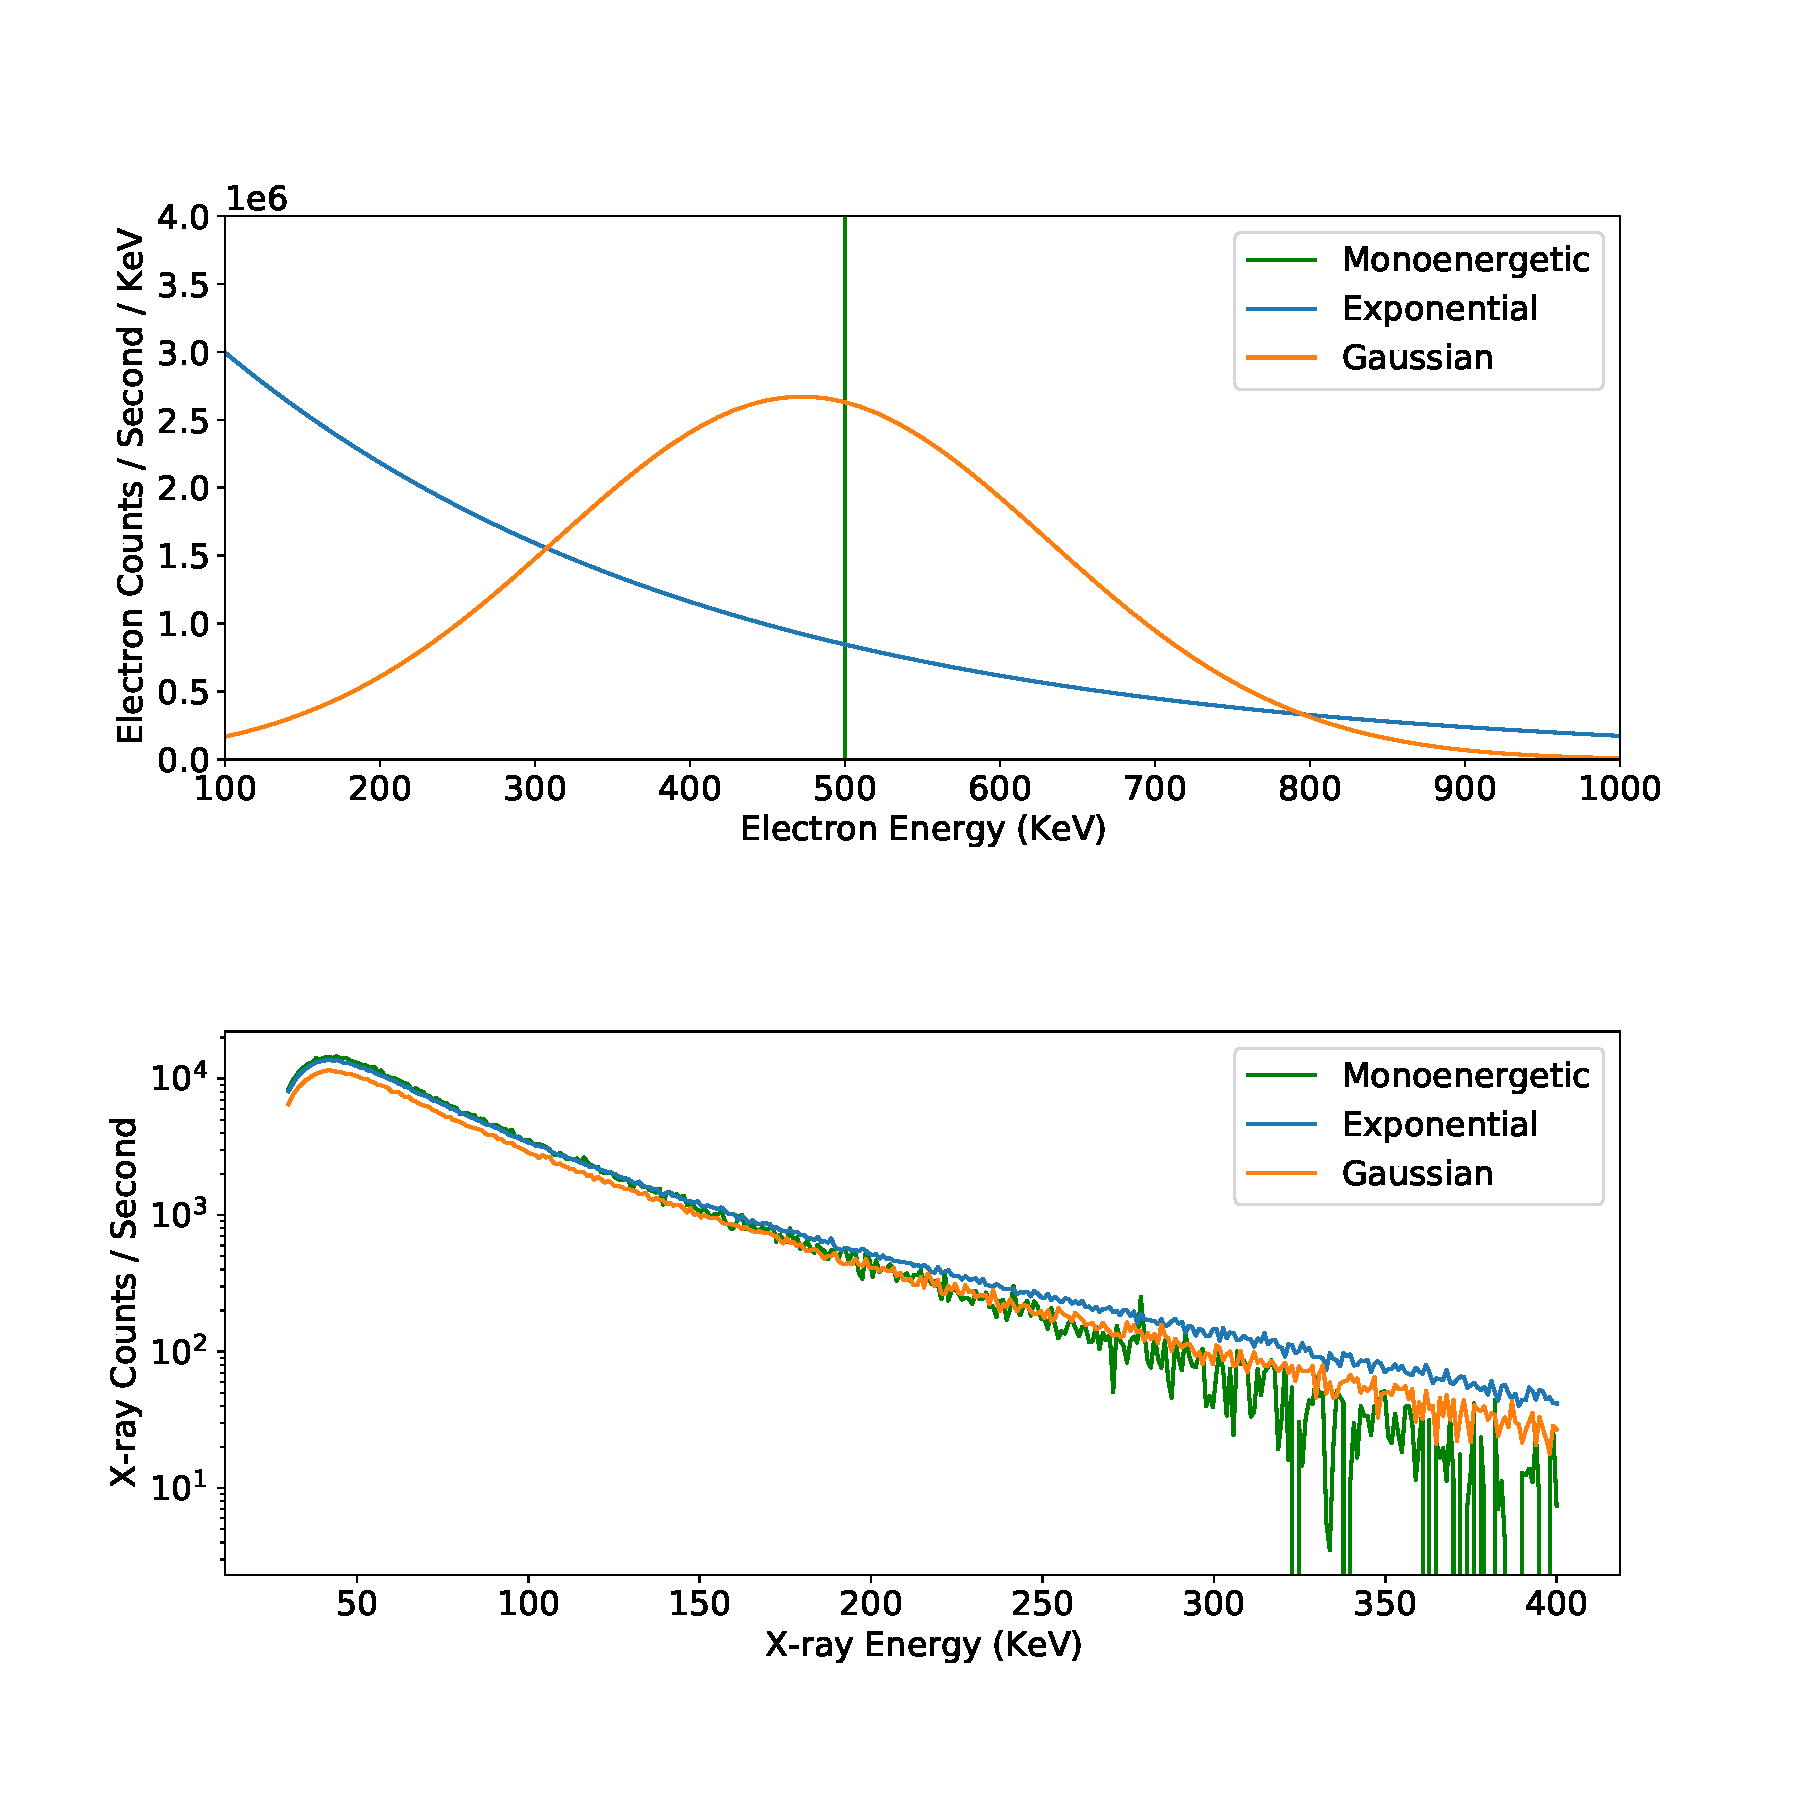
\includegraphics[width=1.0\textwidth]{figures/chapter_4/why_ill_conditioned/fig.pdf}
\caption{(top): Example of three different assumed electron energy spectra (mono-energetic, exponentially decreasing, and gaussian) for a precipitating electron flux of $1\times10^9$ electrons per $\mbox{cm}^2$ per second. (bottom): Resulting simulated X-ray spectra for each electron spectrum, using the methods developed in Chapter 3.} 
\end{figure}

\section{Framing the Inversion Problem}

The forward problem of determining instrument responses from electron precipitation events is linear, and can be written as:

$$\mathbf{G}\mathbf{m} = \mathbf{d}$$

where $\mathbf{G}$ is a matrix representing the discretization of the kernel function mapping precipitating electron spectra $\mathbf{m}$ to resulting measurements of the X-ray spectra $\mathbf{d}$. Techniques for computationally determining $\mathbf{G}$ were discussed in the previous chapter. There is a result that allows the calculation of the condition number of $\mathbf{G}$ as the ratio of its maximal and minimal singular values. As a general rule, if a given linear problem has condition number $\kappa$, then we can expect to lose $10^\kappa$ digits of precision in calculating the solution. This is a best-case estimate, since there will also be round-off errors caused by computer floating point representations of the matrix and the data. Techniques to frame the X-ray inversion problem in such a way as to reduce the effect of the ill-conditioning  of $\mathbf{G}$ will be discussed in the this section.

A representation of matrix $\mathbf{G}$ was developed in Chapter~3 using monte-carlo simulations. In that analysis, a Green's function approach is used to write the X-ray spectra resulting from arbitrary input electron spectra as a linear combination of the effects of mono-energetic electron beams. The dimensions of matrix $G$ are determined by the binning scheme used to represent electron and X-ray energy spectra. For the forward problem, the particular binning scheme chosen for both spaces is not critical, provided it is fine enough to capture the scale of the details of interest in both spectra, but coarse enough to support obtaining adequately pure statistics for the resulting X-ray spectra in a practical amount of computing time. For the inverse X-ray problem, however, the binning scheme chosen for kernel function $\mathbf{G}$ has a critical effect on the conditioning of the inverse problem.

To show the effect of choosing different binning schemes for the rows and columns of $\mathbf{G}$, we plot the condition number as a function of bin widths in KeV for the input electron spectra and output X-ray spectra in Figure~\ref{condition_number_binning}. 

\begin{figure}[p]
\label{condition_number_binning}
\centering
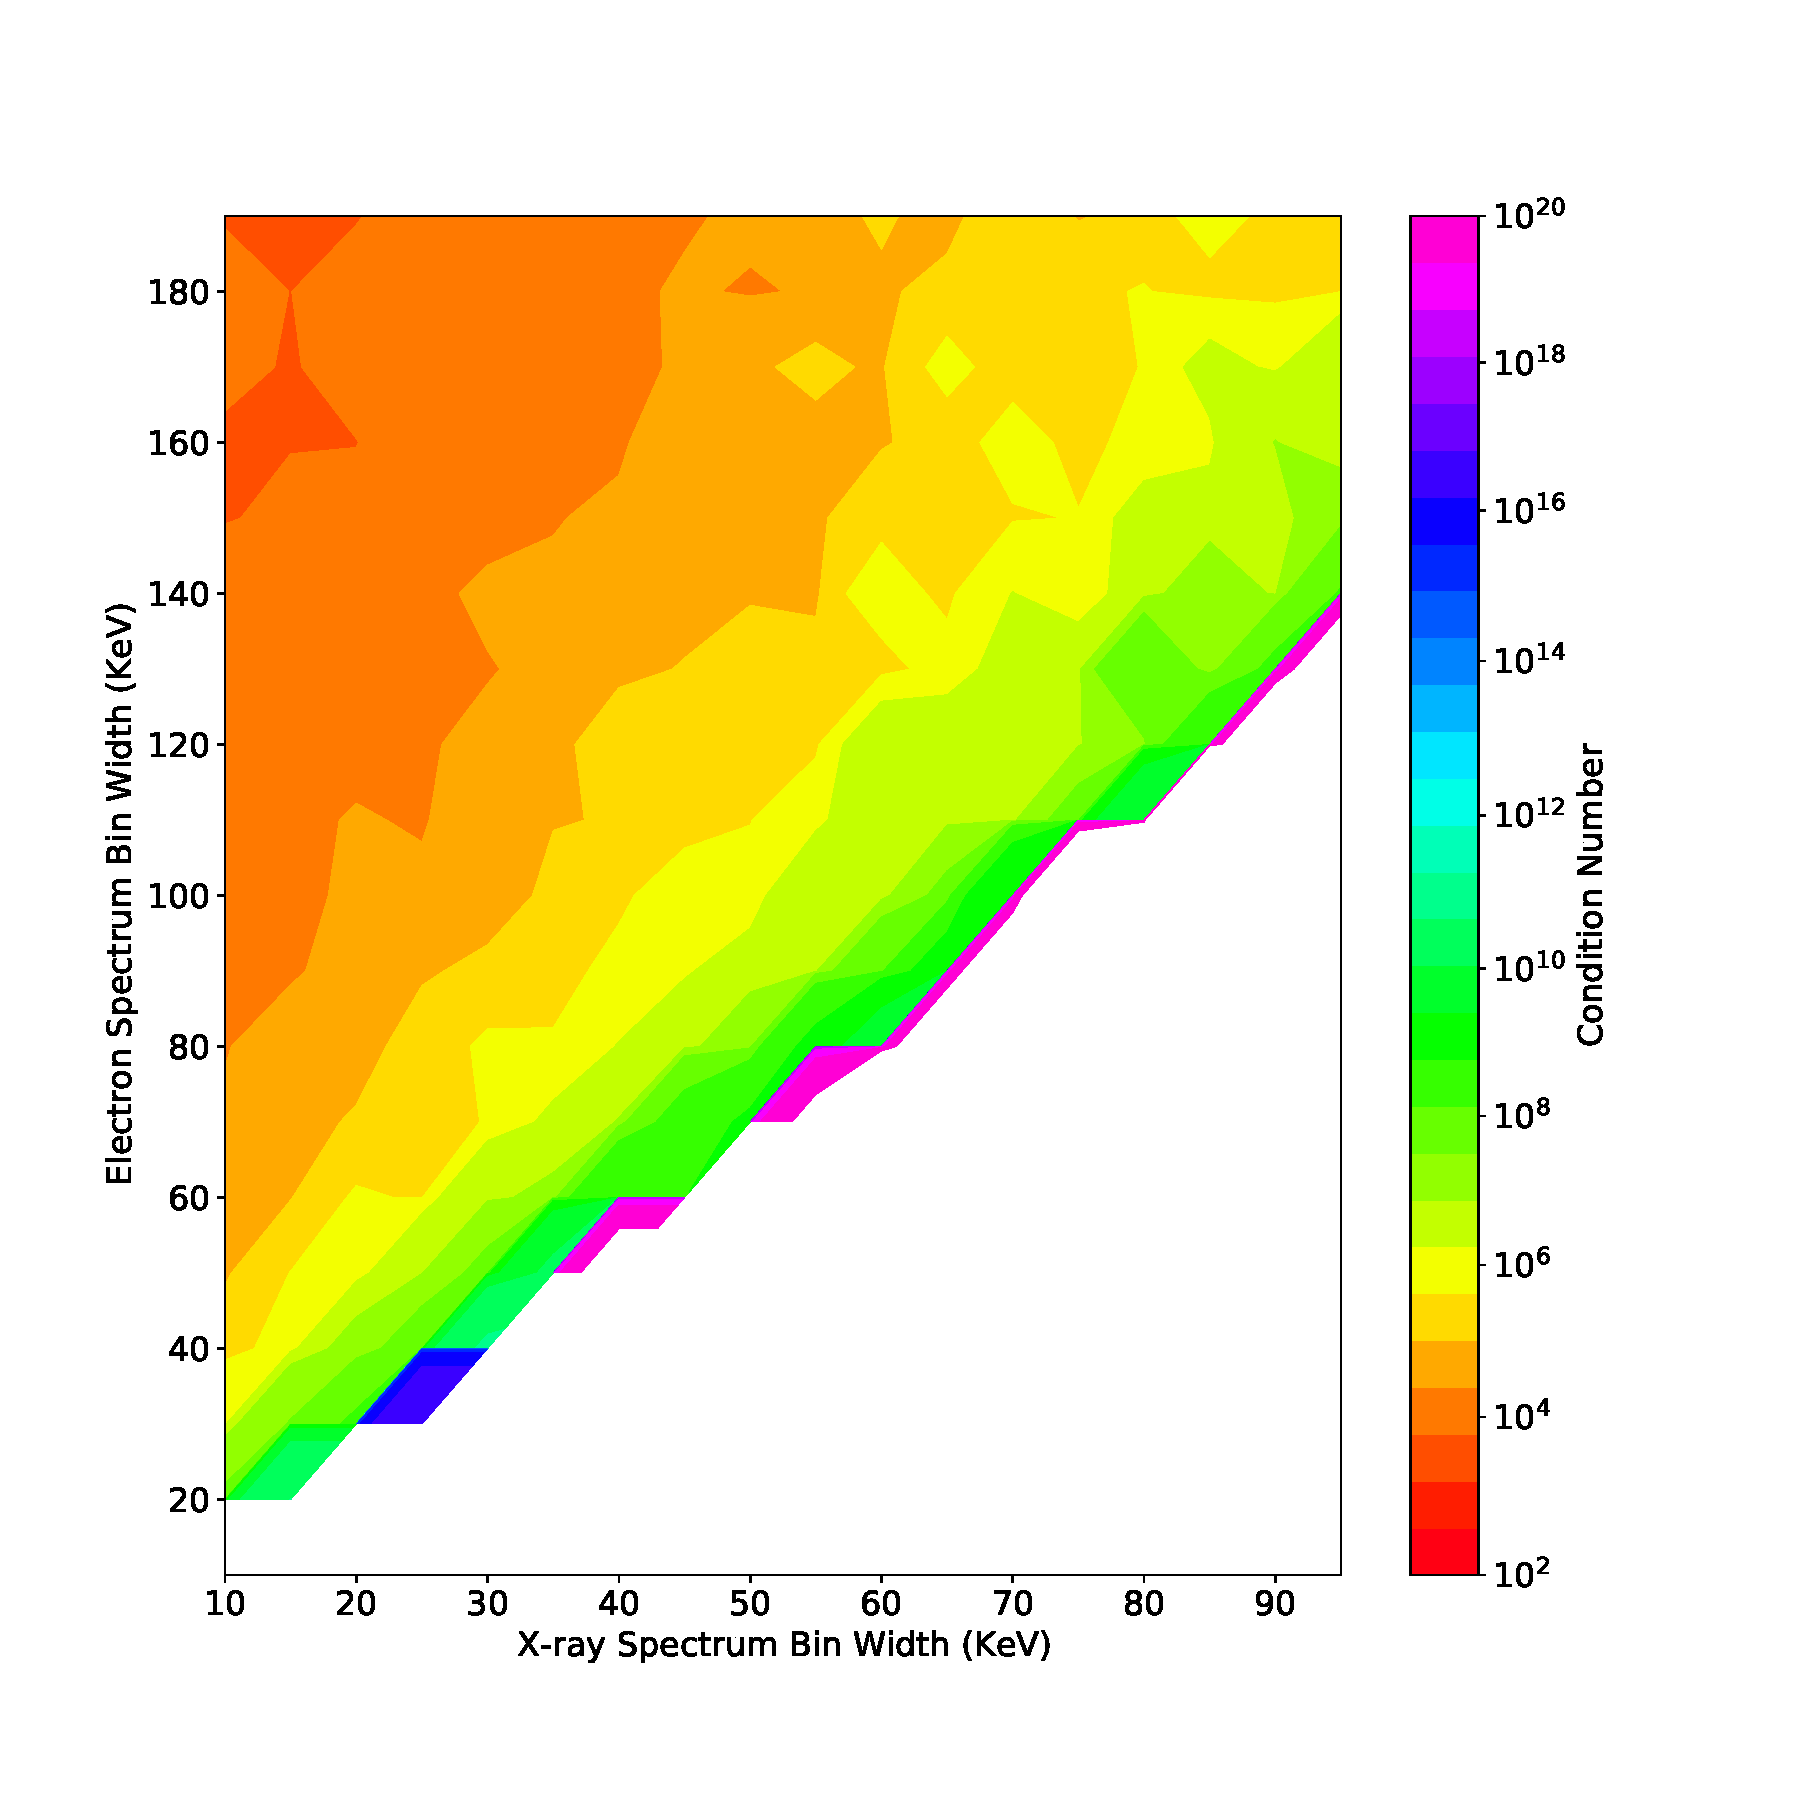
\includegraphics[width=1.0\textwidth]{figures/chapter_4/condition_number_binning/fig.pdf}
\caption{Condition number of mapping $\mathbf{G}$ as a function of X-ray spectrum and electron spectrum bin-widths in KeV. The white region is the domain where the condition number is infinite, and $\mathbf{G}$ is singular.}
\end{figure}

Figure~\ref{condition_number_binning} shows that there is a significant set of bin widths which make $\mathbf{G}$ singular. There are also some general trends apparent. Smaller bin widths for the X-ray spectrum tend to reduce the condition number of the problem, as do larger bin widths for the electron spectra. The results from attempting to solve the inverse problem by directly inverting $\mathbf{G}$ are shown for simulated X-ray and electron spectra across different binning schemes in Figure~\ref{direct_inversion_example}.

\begin{figure}[h]
\label{direct_inversion_example}
\centering
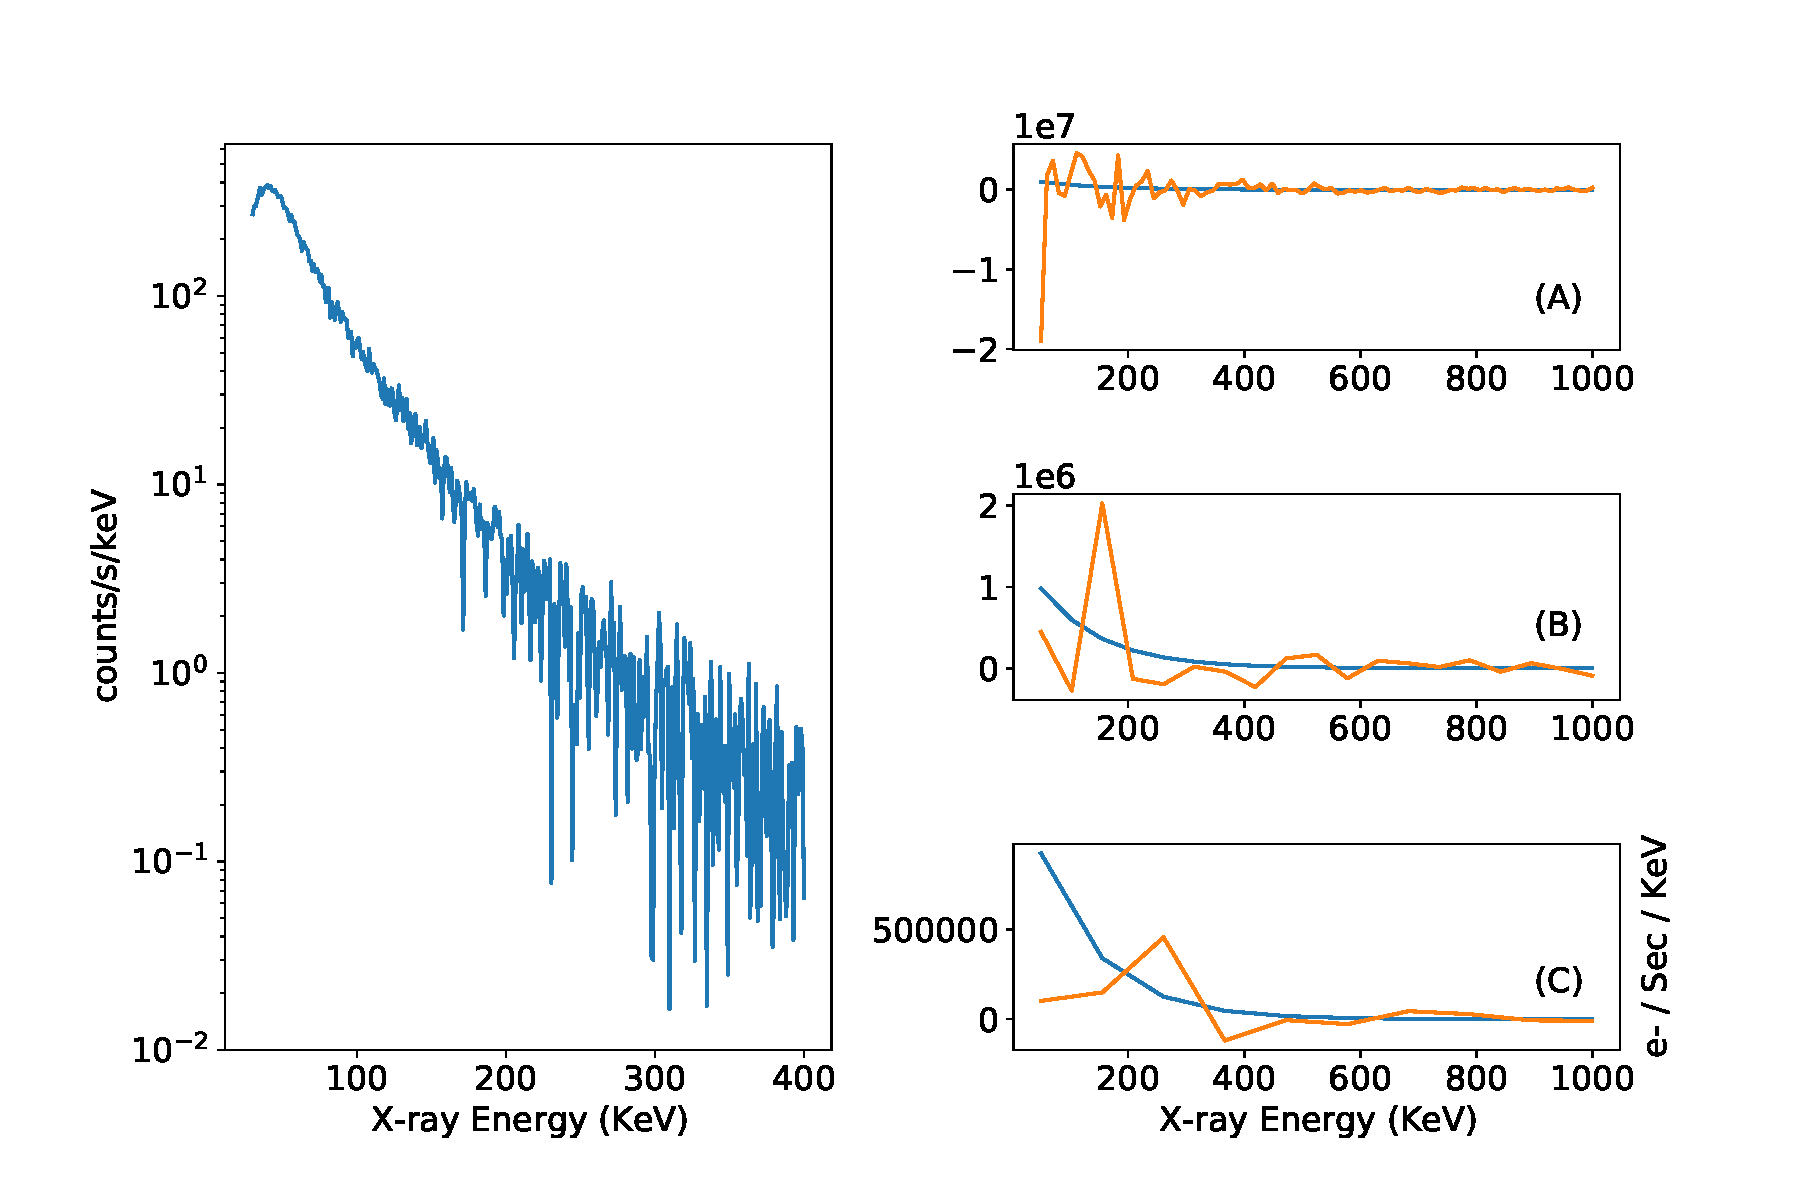
\includegraphics[width=1.0\textwidth]{figures/chapter_4/direct_inversion_example/fig.pdf}
\caption{Direct matrix inversion applied to simulated exponential electron spectra with bin widths of 10 (A), 50 (B), and 100 (C) KeV. The incident particle flux is $1\times10^8$ electrons / second / KeV. }
\end{figure}

The direct inversion attempts in Figure~\ref{direct_inversion_example} are an example of a fundamental trade-off encountered when solving inverse problems. Because the information contained in the available measurements is subset to the information contained in the physical event being studied, the best solution, in terms of minimizing residuals between predictions of the resulting model and the data, often has a high variance and contains little useful information. This corresponds to case (A) in Figure~\ref{direct_inversion_example}, where the electron spectrum bin widths are small enough that the model obtained is mostly random noise. On the other hand, choosing wide bin widths as in case (C) can leave relevant information contained in the measurements out of the model, so that while the variance in the solution is low, the model is still not descriptive of the event being studied. This trade-off can be handled through optimization techniques.

\section{Synthetic Data}

The evaluation of techniques to solve inverse problems often depends on the use of synthetically generated, or simulated, data which correspond to solutions which are already known. For the X-ray inversion problem, synthetic data are readily generated using the monte-carlo techniques discussed in Chapter~3. Since the forward problem is linear, X-ray spectra can be generated which correspond to arbitrary electron spectra using a Greens function approach at little computational expense. This represents a power which can be exploited in the analysis of the problem at hand.  

Realistic synthetic data sets always have an error term added, which must be consistent with the statistics of the experiment being simulated. Measuring X-ray spectra is a counting experiment, and therefore the random error associated with the recorded count for a given energy bin has a Poisson distribution. This distribution can be treated as approximately normal for total counts greater than around 10 in each energy bin. This property can be used to simulate an X-ray spectrum which corresponds to an assumed count rate, by adding appropriate noise to the signal produced using the techniques of Chapter~3.

In a real experiment, a measured X-ray spectrum must be background subtracted. The background subtraction is difficult to simulate and is a source of systematic error. Natural sources such as the 511 KeV annihilation line couple with noise inherent to the detector to make a background energy spectrum with a characteristic shape. We will use a sample drawn from experimental data sets to generate a characteristic background spectrum, and then add an appropriately scaled version to synthetic data generated for a given electron distribution and count rate. This approach neglects any systematic error caused by, for example, detector calibration drifting due to temperature changes. 

Due to the sensitivity of the X-ray inversion problem to small perturbations in the measured spectrum, care must be taken when applying tests using synthetic data so as not to introduce a sampling bias in the measured performance of different inversion techniques. It is possible, for example, to combine a particular background subtraction with a simulated spectrum and corresponding measurement noise to obtain a solution to the inverse problem which very nearly matches the assumed causative electron spectrum. This may not be the case when the same test is subsequently run with a different sample of the background spectrum, or a different random seed for the simulated detector noise. For this reason, single tests of an inversion method on one synthetically generated spectrum have no significance. Evaluating a solution technique to the inverse problem on synthetic data is itself an experiment, and must be treated using a sample size large enough to provide significance in the results. 

The data available for this project was obtained using multiple detectors which all had an identical design (discussed in Chapter~3). Since the data set is large, many background samples can be generated for use when creating synthetic data. An example of a ``quiet time'' X-ray spectrum is shown in Figure~\ref{quiet_time_xray}. Over 20 of these background spectra are collected across the available data set, and used to create the average background spectrum shown in Figure~\ref{quiet_time_xray_average}.

Simulated X-ray spectra which are generated using the techniques of Chapter~3 are created without a background component. To account for this in the generation of synthetic data, the average of the available measured background spectra is added to the simulated spectrum, and then a randomly chosen background spectrum is subtracted. We will assume that the differences across all of the measured background spectra can be used as a proxy for the systematic error
expected when a particular background subtraction is applied. 

The complete procedure to conduct a test on an inversion method using synthetic spectra is therefore: 

\begin{enumerate}
    \item An expected X-ray spectrum resulting from an assumed electron distribution is generated using the simulations of Chapter~3. 
    \item Normally distributed noise is added with a standard deviation corresponding to the assumed total X-ray count rate.
    \item The average background spectrum from the available experimental data is added.
    \item A particular background spectrum from the set of experimental data is subtracted.
    \item This process is repeated across the different measured background spectra and across different random seeds for the generated noise, to create a set of synthetic X-ray spectra.
    \item The inversion method being examined is applied across the set of synthetic X-ray spectra, and the resulting inversions are compared statistically with the assumed electron distribution. 
\end{enumerate}

This procedure generates results for one test on a particular inversion method for a particular assumed spectrum. To evaluate the performance of a given inversion method, this entire procedure needs to be repeated across many different assumed causative electron distributions. While the generation of a particular synthetic data set is computationally cheap, the evaluation of the inverse problem can be expensive depending on the technique used. It is, however, absolutely essential that the evaluation of different inversion methods be carried out across a wide data set to avoid sampling bias. This is even more critical when the inversion method being studied is adaptive, depending on the noise level of the input data set. For this case, the entire procedure must be repeated again across different synthetic spectra corresponding to the range of possible count rates.  

There needs to be an objective measure for the relative performance of a given inversion method. The metric should be a scalar, and should increase with the amount of detail that the inversion method captures about the assumed electron spectrum when it is applied to synthetic data. The normalized mean squared error (NMSE) is a simple metric which satisfies these properties. The NMSE is the squared total difference between the retrieved electron spectrum and the assumed electron spectrum, but normalized to the total signal magnitude to account for the fact that it is applied across different count rates. The definition follows.

\begin{definition}[NMSE]
The normalized mean squared error between assumed spectrum $\mathbf{y'}$ and expected spectrum $\mathbf{y}$ is: 

$$\mbox{NMSE}(\mathbf{y},\mathbf{y'}) = \frac{\vert \vert (\mathbf{y} - \mathbf{y'}) \vert \vert}{\vert \vert \mathbf{y} \vert \vert}$$.
\end{definition}

The NMSE is zero for a perfect agreement between a simulated and retrieved electron spectrum, and increases as the agreement becomes worse. Tests on different inversion techniques will produce distributions of the NMSE. These distributions, and particularly their mean and variance, will be the objective measures used for comparing inversion techniques. 

\section{The Least-Squares Regression and the Bias-Variance Trade-off}

Due to the ill-posed nature of the X-ray inversion problem, solutions often take the form of \textit{estimators}. These estimators may be either unbiased, as in the case of least-squares regression, or contain a bias term towards solutions with chosen properties. In Figure~\ref{why_ill_conditioned}, it is apparent that directly solving the X-ray inversion problem using least-squares regression can be ineffective. This is because the problem has a high condition number (Figure~\ref{condition_number_binning}). There is a trade-off apparent for this problem: the condition number can be reduced by selecting coarse binning in model space, which reduces the variance in the solution, but also reduces the amount of information about the data the solution represents. The optimization of this trade-off for a given data set is a basic and well-understood problem in data analysis. A solution is said to be \textit{over-fit} when it aligns well with one data set, but fails to usefully describe the data under small perturbations or additional measurements. On the other hand, a solution is \textit{under-fit} when it fails to reflect significant changes in measurement data. 

Determining the balance between over-fitting and under-fitting a given data set is a basic and well-understood problem in data analysis. Roughly speaking, the variance in the data set is used as a proxy for how much variance is expected in well-fit models which describe the data. The $\chi^2$ statistic is a standard descriptor for this relative variance.

\begin{definition}[$\chi^2$ Statistic]
The $\chi^2$ statistic is the quantity 

$$\chi^2 = \sum_i \frac{(O_i - E_i)^2}{\sigma_i^2}$$

where $\mathbf{O_i}$ are the observed, or measured quantities, $\mathbf{E_i}$ are the expected, or model, quantities, and $\sigma_i^2$ are the variances in the measured quantities. 
\end{definition}

The $\chi^2$ statistic is usually normalized to the number of degrees of freedom which a particular problem has, which gives the reduced $\chi^2$ statistic.

\begin{definition}[Reduced $\chi^2$ Statistic]

The reduced $\chi^2$ statistic is the $\chi^2$ per degree of freedom, $\nu$: $$\chi^{2}_\nu = \frac{\chi^2}{\nu}.$$

\end{definition}

If the reduced $\chi^2$ statistic is much greater than 1, then it indicates a poor model fit. When the  reduced $\chi^2$ statistic is much less than 1, it indicates over-fitting to the data. An example of this is shown in Figure~\ref{overunderfit_example} for polynomial models fit to a randomly generated data set.

\begin{figure}[p]
    \centering
    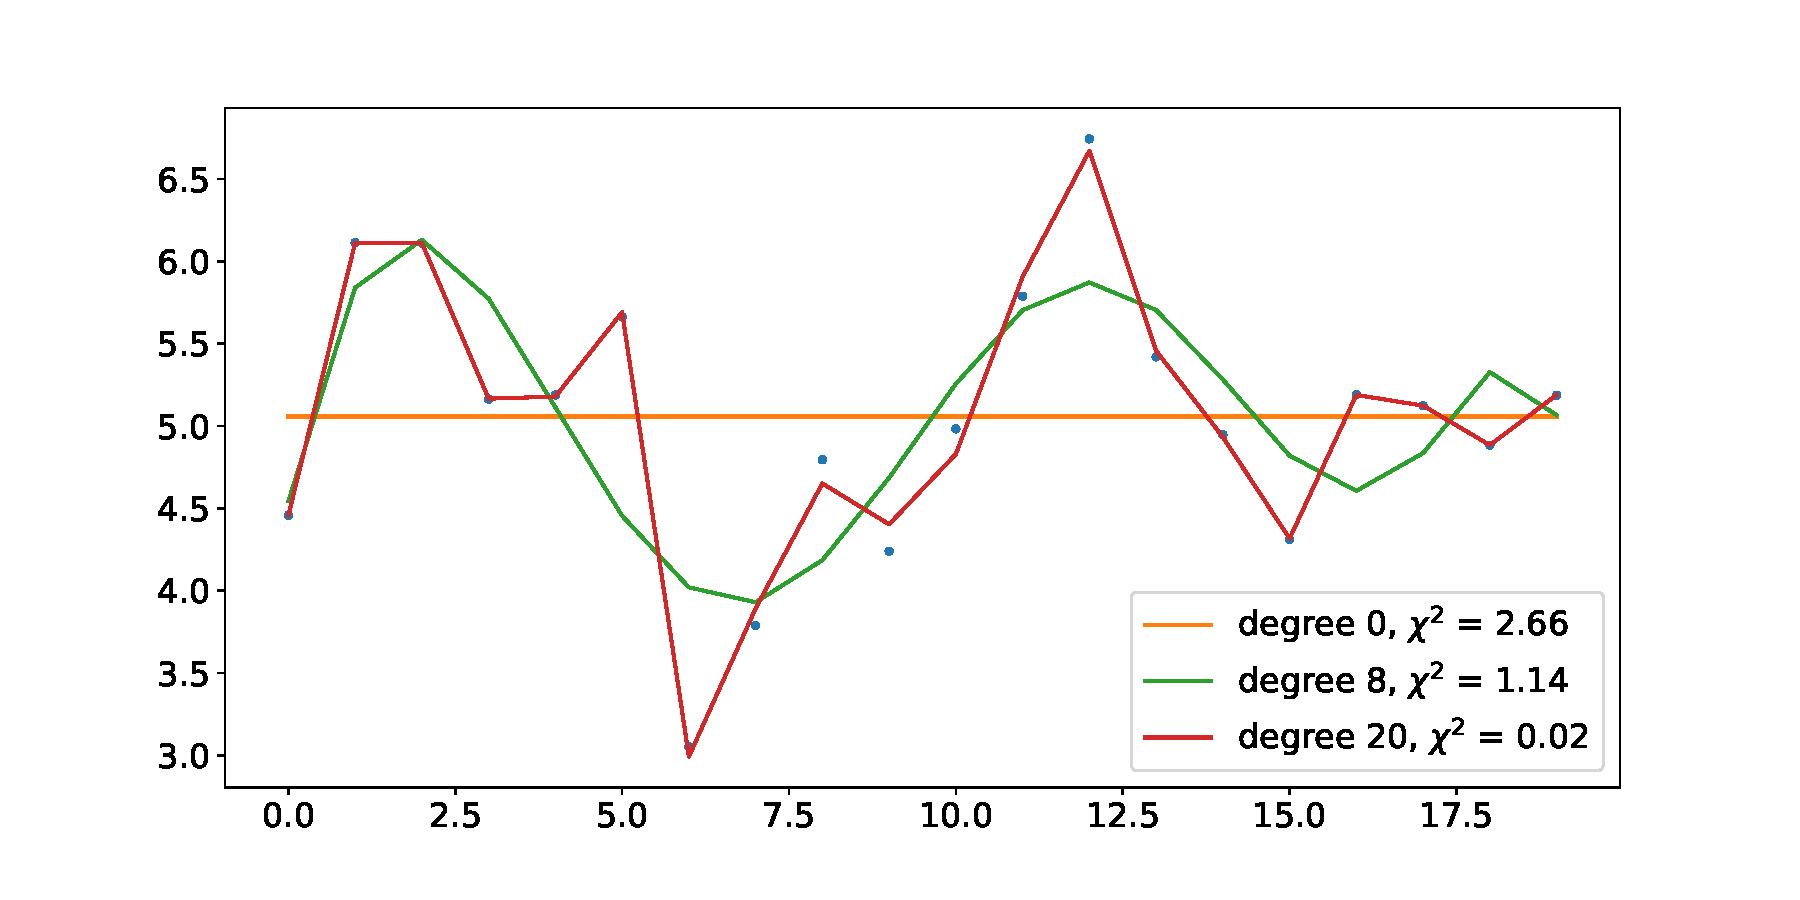
\includegraphics[width=1.0\textwidth]{figures/chapter_4/overunderfit_example/fig.pdf}
    \caption{Example of over-fit and under-fit models to data. A random data set is generated and polynomial models are fit using least-squares regression. The reduced $\chi^2$ statistic is shown for each model.}
    \label{overunderfit_example}
\end{figure}

Managing the balance over-fitting and under-fitting models is related to the condition number of the problem at hand. If a problem is badly conditioned, as with the X-ray inversion problem, then it may be necessary to under-fit the data to get any useful information from the solution. An example which frequently occurs in test inversions on test data is the existence of negative particle fluxes in predicted electron spectra, an example of which can be seen in Figure~\ref{why_ill_conditioned}. There is no clear way to interpret models with these features. Eliminating them from predicted models is possible using constrained optimization techniques, and will be discussed in the next section. Constrained optimization, combined with other modifications to the least-squares estimator to improve conditioning of the X-ray inversion problem, will be the topic of the remainder of this chapter. 

\section{Biased Estimators and Improving the Condition Number}

The condition number for a given linear problem can be expressed as the ratio of the maximum and minimum singular values in the kernel matrix. Using the singular value decomposition, it is possible to write an alternative version of the X-ray inversion problem with smaller singular values suppressed or removed. The singular value decomposition writes the kernel matrix $\mathbf{G}$ as:

$$\mathbf{G} = \mathbf{U}\Sigma\mathbf{V^T}$$

where $\mathbf{U}$ and $\mathbf{V}$ are unitary, and $\Sigma$ is a diagonal matrix with the singular values on the diagonal. Since the decomposition can be chosen such that the singular values are in descending order, an approximation and reduction in dimensions to the original kernel matrix can be generated by truncating the expansion. Processes like this produce biased estimators, or imperfect representations of data represented by the kernel matrix, in exchange for more solution stability. In this section we will examine the effects of these approximations on the X-ray inversion problem using synthetically generated data from the techniques of Chapter 3. 

Figure~\ref{condition_number_binning} shows that the best binning scheme for the X-ray inversion problem kernel matrix minimizes the bin sizes for the data (X-ray spectra), and maximizes the bin size for the models (electron spectra). This choice must be made within the limits of the statistics of the data set at hand, and the amount of detail desired in the model electron spectrum. As discussed in the previous section, the $\chi^2$ statistic is used to avoid over or under-fitting the problem. Unfortunately, this result is valid only for unbiased estimators, such as the least-squares regression. For a biased estimator, determining the right solution size becomes a much more complicated problem that will be addressed in the next section.

Figure~\ref{singular-value-plots} shows the distribution of singular values across different electron spectrum bin widths. The X-ray spectrum bin widths are left at 1 KeV. Most of the information contained in the kernel matrix is captured in the first few terms of the singular value decomposition. This suggests that reducing the dimensions of the problem by truncating the singular value decomposition might improve its condition.

\begin{figure}[p]
    \centering
    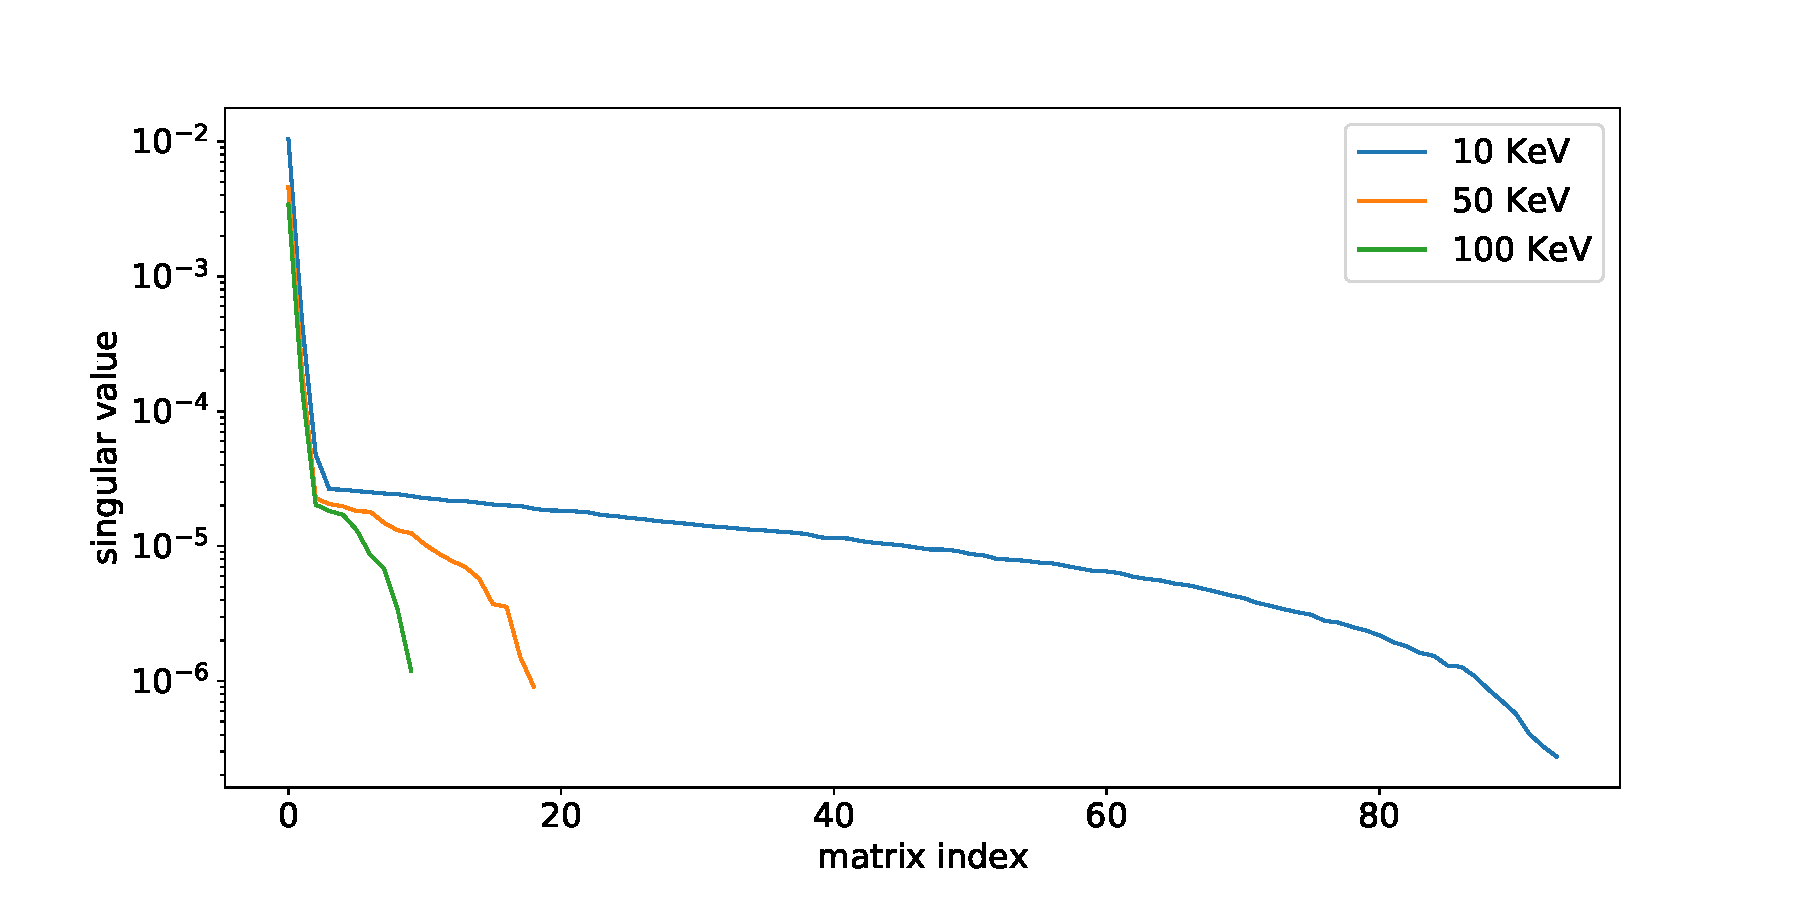
\includegraphics[width=1.0\textwidth]{figures/chapter_4/singular_value_plots/fig.pdf}
    \caption{Plots of the singular values of the kernel matrix for the X-ray inversion problem for different electron spectrum bin widths, with singular values arranged from biggest to smallest.}
    \label{singular-value-plots}
\end{figure}

To justify the use of a biased estimator in solving the X-ray inversion problem, two questions need to be answered. The first is whether or not the use of the biased estimator significantly improves the conditioning of the problem. The second is whether the bias significantly degrades the amount of information contained in the solutions. The first question is easily answered by graphing the condition number of the kernel matrix as a function of truncation index. This is shown as a function of binning scheme in Figure~\ref{condition-number-binning-tsvd}.  

\begin{figure}[p]
    \centering
    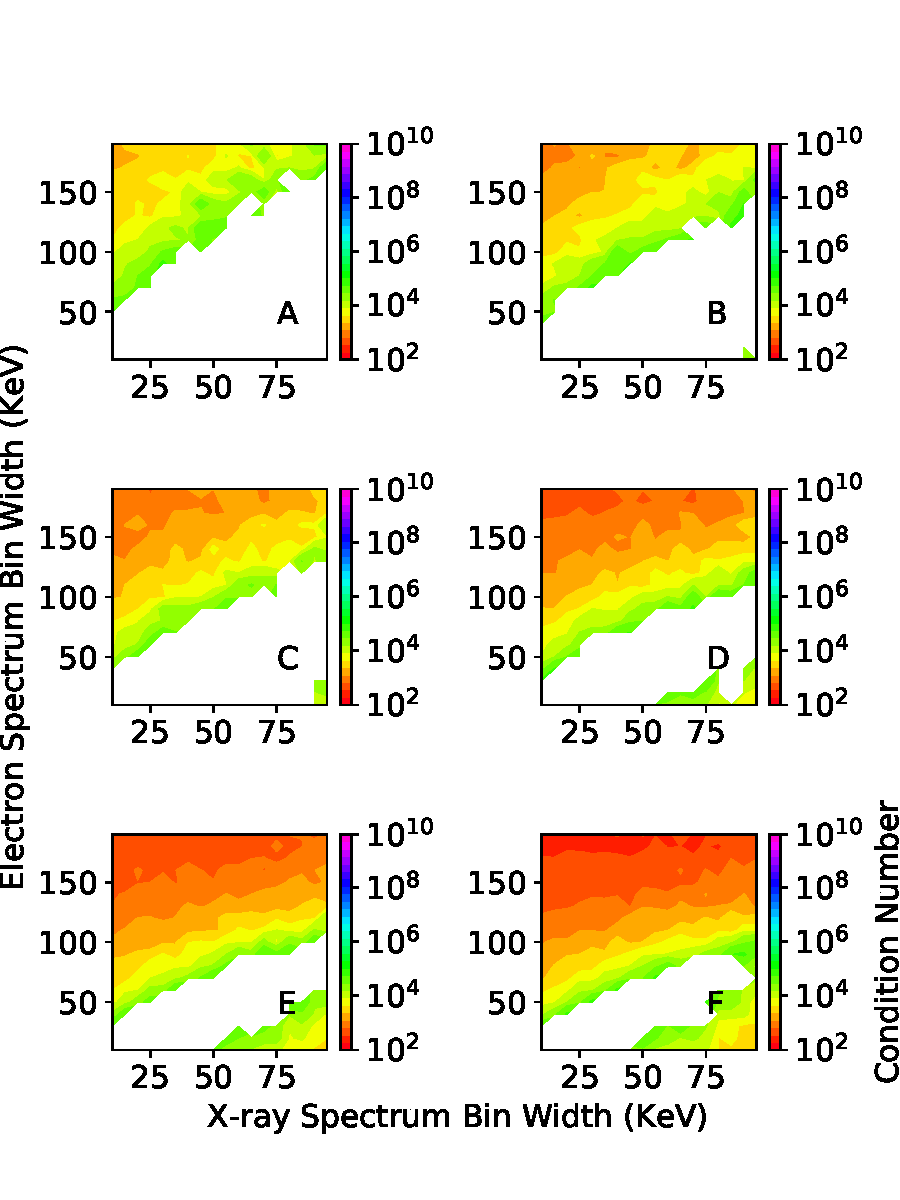
\includegraphics[width=.95\textwidth]{figures/chapter_4/condition_number_binning_tsvd/fig.pdf}
    \caption{Plots of the condition number of the kernel matrix for the X-ray inversion problem as a function of electron spectrum and X-ray spectrum bin width, for 1 (A) through 6 (F) truncated singular values.}
    \label{condition-number-binning-tsvd}
\end{figure}

Compared to Figure~\ref{condition_number_binning}, the plots in Figure~\ref{condition-number-binning-tsvd} show that truncating the smallest singular values of the kernel matrix has a positive effect on the conditioning of the X-ray inversion problem. The number of binning schemes which produce a singular kernel matrix, with no inverse, is reduced with increasing truncation index. In addition, the regions with low condition numbers where the inverse problem is tractable (less than $10^3$) are expanded. 

The improved conditioning of the inverse problem by truncating small singular values comes at a significant cost by introducing solution bias. There is no simple method to describe the amount of bias this process introduces, or the effect it will have on a particular data set, however, we can apply the least squares inversion to sample data, as in ~\ref{why_ill_conditioned}, using the truncated kernel and see what effect the bias has. 

Before applying a biased estimator to the inversion problem, there is an important fact which must be made explicit. The main symptom of an ill-conditioned problem is a high sensitivity to small perturbations on the input data. Because of this, one obtains almost no information about the overall behaviour of a given estimator on the X-ray inversion problem by running single tests on synthetic data (which can be generated using the techniques of Chapter 3.) X-ray measurements are counting experiments, and they are subject to statistical noise in their measurements. The statistical noise will follow a Poisson distribution in a well-designed experiment without significant uncorrected detector bias. Since the data have a random component, it would be an error in methodology to attempt to solve the X-ray inversion problem on one specific instance of synthetically generated data. Rather, one should sample a given synthetic data set many times, and then use the inversion technique of choice to see the resulting distribution of computed electron spectra. 

This technique is applied to synthetic electron spectra in Figure~\ref{tsvd_test}. Exponential electron distributions and their resulting X-ray spectra are simulated, and then the X-ray inversion problem is solved using the truncated singular value decomposition and least-squares regression for different truncation indices. The stabilizing effect the truncated SVD approximation has on solutions to the X-ray inversion problem is apparent, though, it is important to note that the spread in the reconstructed spectra due to statistical noise in the simulated X-ray measurements remains significant. In a real experiment, one obtains only one measurement of the X-ray spectrum and the underlying statistical distribution in the noise. This presents a significant problem for reconstructions based on biased estimators, since there is no a-priori way to predict how their characteristic bias will map the noise statistics in measurement space to model space. Despite this problem, and the associated difficulty assigning meaningful error estimates to reconstructed spectra, Figure~\ref{tsvd_test} motivates the search among biased estimators for solutions to the X-ray inversion problem. It is entirely possible, for example, that a measured X-ray spectrum has statistics which only support a binning scheme which makes the inverse problem impossible. A biased estimator, such as truncated singular value decomposition, which effectively improves solution resistance to noise, can be the only way to recover a useful model in these scenarios. 

The use of the truncated singular value decomposition as a biased estimator introduces the truncation index as a free parameter. This leads to an important question: when is the problem well-conditioned enough for the data set being analysed? Higher degrees of truncation improve the conditioning of the X-ray inversion problem (Figure~\ref{singular-value-plots}), but only at the cost of less information being represented in the inverse mapping. The introduction of a free parameter which controls the bias-variance trade-off is a general feature of biased estimators used to solve inverse problems. This too represents a cost, since the choice of this free parameter must be somehow justified. The question then becomes whether there is a method to choose this parameter based on data from a given experiment. This question is central to the X-ray inversion problem, and is the focus of the remainder of this chapter. 

\begin{figure}[p]
    \centering
    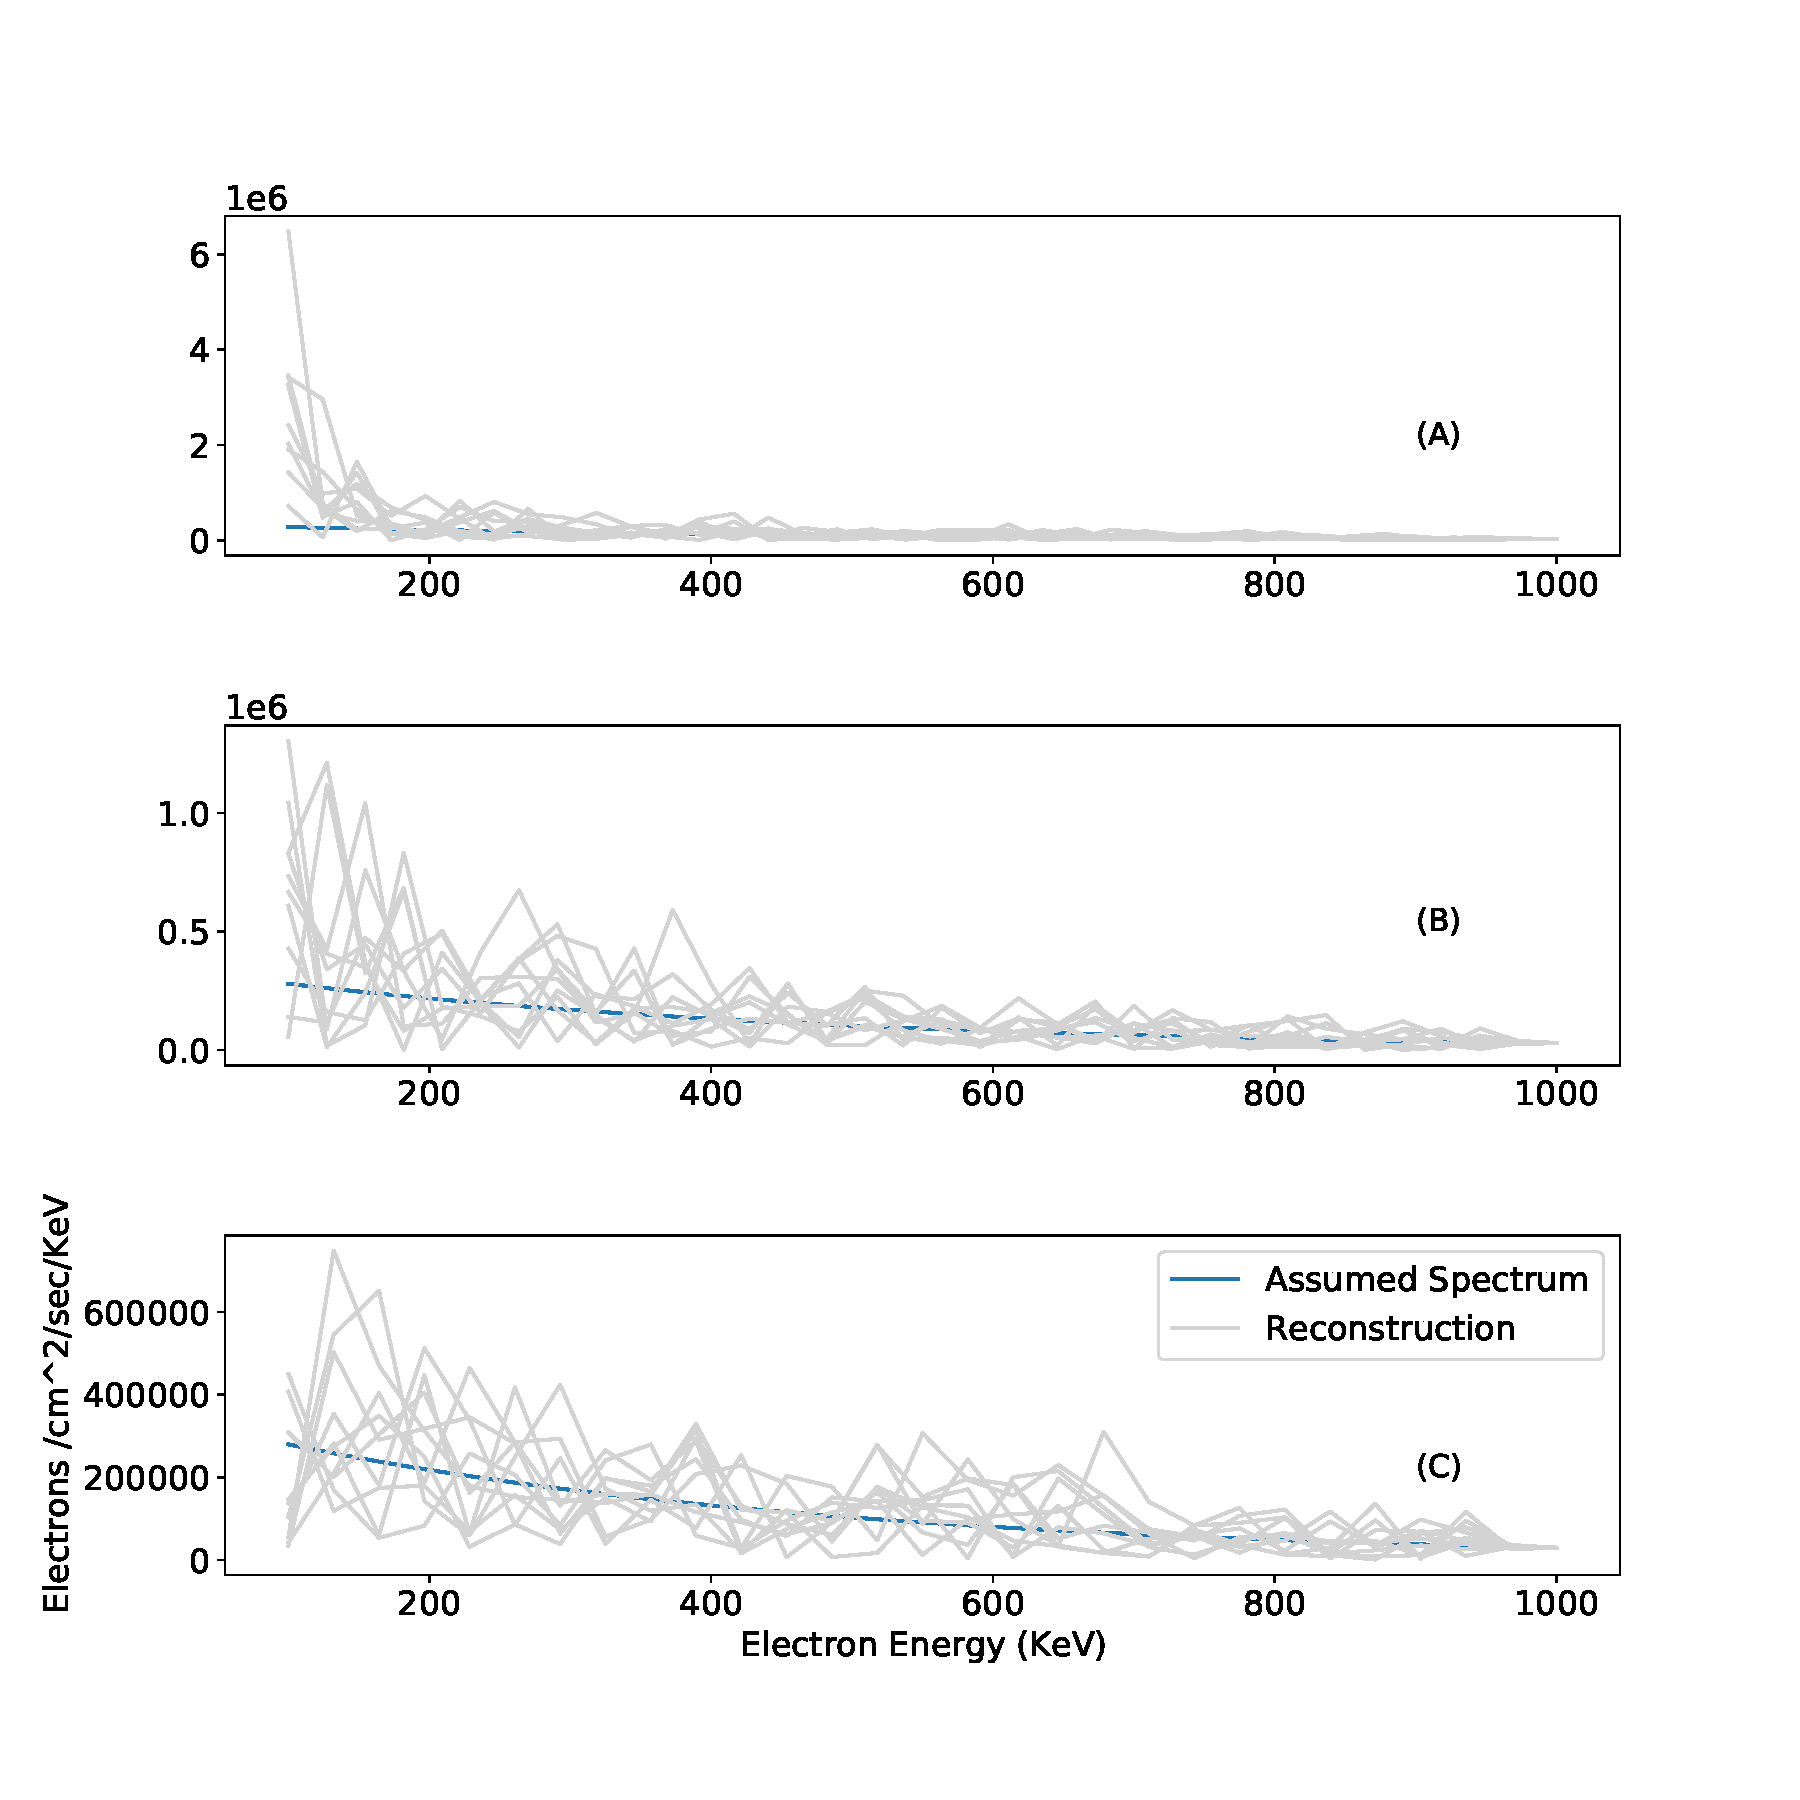
\includegraphics[width=.95\textwidth]{figures/chapter_4/tsvd_test/fig.pdf}
    \caption{Plots of simulated electron spectra for a total electron flux of $1\times10^9 \mbox{electrons} / \mbox{cm}^2 / \mbox{second}$, and their reconstruction from the associated simulated X-ray spectra using a truncated singular value approximation of the kernel matrix. Electron bin widths are set to 50 KeV, and X-ray bin widths to 1 KeV. (A), (B), and (C) show reconstructions with the smallest 1, 5, and 10 singular values dropped from the expansion.}
    \label{tsvd_test}
\end{figure}

\section{Tikhonov Regularization and the L-Curve Method}

The truncated singular value decomposition explored in the last section is not the only method which has been developed to recondition inverse problems. For the optimization problems that arise from the introduction of a free parameter with biased estimators, it is desirable to have a continuous variable which controls the degree of reconditioning, rather than a discrete truncation index. Further, it is useful to have an estimator which exhibits a bias towards certain families of solutions, using a-priori knowledge we might have about the shape of the expected solution to the inverse problem. The method of Tikhonov regularization has these properties.

In Tikhonov regularization, the unbiased least-squares regression:

$$\min_{\mathbf{x}} \vert \vert \mathbf{A} \mathbf{x} - \mathbf{b} \vert \vert $$

is replaced with the modified version:

$$\min_{\mathbf{x}} \vert \vert \mathbf{A} \mathbf{x} - \mathbf{b} \vert \vert + \alpha \vert \vert \mathbf{x} \vert \vert.$$

The parameter $\alpha$ is a positive real number which controls the strength of the regularization. When $\alpha$ is zero, the least-squares solution is recovered. The addition of $\alpha \vert \vert \mathbf{x} \vert \vert$ to the least-squares minimization represents a penalty term on the size of the solution norm. There is a close relationship between the effect of adding this penalty term and the suppression of small singular values in the kernel matrix. Write the singular value decomposition of the kernel matrix as:

$$\mathbf{G} = \mathbf{U}\Sigma\mathbf{V^T}.$$

It can be shown that the solution to the Tikhonov regularization can be written as:

$$\mathbf{x} = \mathbf{V}\mathbf{D}\mathbf{U}^T \mathbf{b} $$

where the diagonal values of $\mathbf{D}$ are:

$$\mathbf{D_{ii}} = \frac{\sigma_i}{\sigma_i^2 + \alpha^2}$$

where $\sigma_i$ are the singular values of $\mathbf{G}$. The regularization term applies a filtering effect which smoothly suppresses the smallest singular values in the kernel matrix. This effect improves the condition number of the kernel matrix, and stabilizes solutions to the inverse problem. This is accomplished at the cost of a bias towards solutions with a small norm, which scales with the degree of regularization applied. 

Tikhonov regularization has a heuristic interpretation. The deviation from a solution with a small norm can be viewed as a measure of its complexity, and the amount of information which it contains. The trade-off between solutions to inverse problems with stability but high bias, and solutions with small residual errors but high variance, is controlled by the regularization parameter $\alpha$. There is no single method to choose an appropriate value for $\alpha$ for a given problem. Techniques to select $\alpha$ can include heuristic arguments, a-priori knowledge based on the properties of the particular problem at hand, and statistical arguments. Combinations of these methods are also possible, but all of them represent an implicit cost to the analysis of the problem at hand, namely, that a choice in $\alpha$ ultimately needs to be made, and that choice will always depend, to an extent, on the preferences of the analyst. This is a danger to the analysis of the X-ray inversion problem, which we will mitigate through careful testing on synthetic data across multiple techniques, and objective scoring of different techniques using clearly defined metrics. 

The classic method for choosing $\mathbf{\alpha}$ is the so-called ``L-curve''. This heuristic method works by plotting the solution norm $\vert\vert \mathbf{x} \vert\vert$ vs the error term $\vert \vert \mathbf{A}\mathbf{x} - \mathbf{b} \vert \vert$ in log-log space. Typically, but not always, this plot has a characteristic L shape, with an inflection point which locates the value for $\alpha$ that produces the most significant reduction in solution norm for the smallest error term. If the error term is thought of as the cost of solution stability, then the inflection point locates the most economical value of $\alpha$. 

An example of this applied to the X-ray inversion problem is shown in Figure~\ref{l-curve-example}. We use a synthetic X-ray spectrum based on an exponential beam of electrons with a folding energy of 300 KeV. The L-curve is shown and used to select $\alpha = 2.0\times10^{-5}$. The assumed electron spectrum is plotted along with spectra determined using direct matrix inversion, and Tikhonov regularization for the selected value of $\alpha$. Multiple runs across synthetic data generated with different random seeds are used to provide an accurate representation of the variance in each solution. 

\begin{figure}[h]
    \centering
    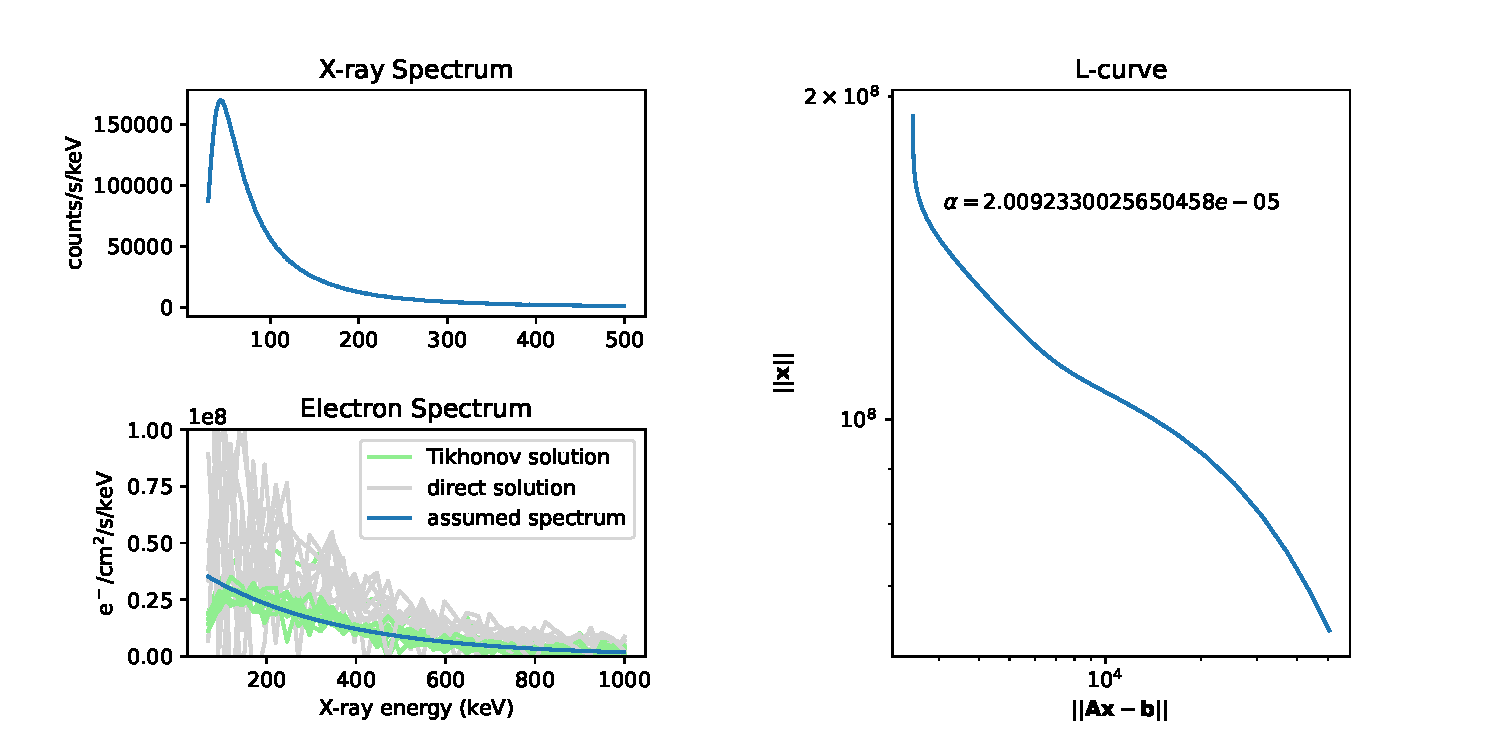
\includegraphics[width=1.1\textwidth]{figures/chapter_4/l-curve-example/fig.pdf}
    \caption{Application of Tikhonov regularization and the ``L-curve'' method to synthetic exponential electron spectrum. The assumed electron spectrum is shown in blue (bottom, left), and the retrieved spectra are shown for direct inversion (grey) and Tikhonov regularization (green).  }
    \label{l-curve-example}
\end{figure}

The reduction in variance gained from the regularization process is evident in Figure~\ref{l-curve-example}. The spread in solutions using direct inversion is large enough, that besides a general trend towards a decrease with lower energies, few other features are readily apparent. Additionally, some of the direct solutions show negative particle fluxes in the lower energy bins. Without careful analysis of the variation in solutions caused by the counting statistics, inversions attempted using experimental data could even be misleading, showing apparently significant features which are in fact only caused by the mapping of random noise through the ill-conditioned kernel matrix of the problem. 

The bias introduced by regularization is also apparent in Figure~\ref{l-curve-example}. Towards lower energies the solution trends downward, which is a feature the assumed electron spectrum does not have. The spectrum retrieved using regularization is also not fully exponential, and a folding energy retrieved by fitting an exponential curve would have a non-zero error when compared with the assumed data. Although the variance in the direct solution is large enough to be untenable when applied to experimental data, it remains exponential, and on average, the folding energy will match the assumed model. 

Unfortunately, there is no general method to assign useful confidence intervals to solutions from biased estimators, including those generated from Tikhonov regularization. The effect of the variance in solutions is simple enough to capture, as done in Figure~\ref{l-curve-example} by running the inversion multiple times under different random seeds, but a true confidence interval would include the effects of both the bias and the variance in the solution. The use of a biased estimator such as Tikhonov regularization  makes an otherwise unsolvable problem tractable, but only at the cost of the certainty and bounds we can place on the solutions. In a way, an ill-posed problem represents a mismatch between the amount of information contained in the solution, and the amount of information in the available data. Tikhonov regularization allows us to control the manifestation of this fundamental lack of information, but there is no process by which it can be eliminated. 

For all the caveats and drawbacks which come with applying Tikhonov regularization to a problem, it has a critical property which the unbiased methods lack - namely that it is \textit{adaptive}. The method works by balancing the variance in the solution against the norm, which means that as data become noisy and harder to resolve, the bias is increased to compensate and maintain stability. This is in sharp contrast to, for example, choosing a binning scheme or parameterization which remains fixed for a given problem. Some data sets are ``easier'' to invert through a given kernel matrix than others, which can be for a multitude of reasons. For example, the data set could represent a monochromatic solution, which incurs the least variance-inducing resistance in the inversions. Tikhonov regularization is sensitive to this fact, and the L-curve will have a shape which corresponds to the particular problem and particular data set at hand. 

The L-curve method is computationally expensive, since solutions need to be generated for every value of $\alpha$ being examined. For relatively small matrices, say, less than 1000 by 1000 rows and columns, this is a small problem, but it becomes significant as the problem being examined scales. Because of this, when using Tikhonov regularization, the most sensible binning scheme for the X-ray inversion problem is not necessarily the one which provides the finest resolution in X-ray spectra, as Figure~\ref{condition_number_binning} would suggest. Practical considerations based on computational limits need to be taken into account. 

The fact that the L-curve method is somewhat heuristic motivates us to look for another way to select a value for $\alpha$. The ``corner'' of the L-curve plot, if it appears, is not always sharp. This represents a way that the expectations of the human doing the analysis can find their way into the solutions created using Tikhonov regularization. There is a family of related methods which can be used to select $\alpha$ based on the statistical properties of the data alone. The cross-validation methods use the idea that the artificial removal of parts of the input data produce different solutions and can give information about the stability of the problem being analysed. In particular, under the hypothesis that the effect of the removal of a single data point, such as a single energy bin in the X-ray inversion problem, should have only a small effect on the retrieved electron spectrum. Iterating over the available energy bins, and suppressing each one from the problem in turn, will produce a spread of solutions, whose variation gives a picture of the overall stability of the inversion. If this entire process is repeated over different values of $\alpha$, then the total mean squared error between the suppressed data points and the regularized solutions is can be compared and minimized. This process is motivated schematically in Figure~\ref{cross_validation_motivation}. In both the over-fit and under-fit cases, the missing data point is fit poorly. Minimizing this effect represents a balance between these cases and produces a corresponding value for $\alpha$. 

\begin{figure}[p]
    \centering
    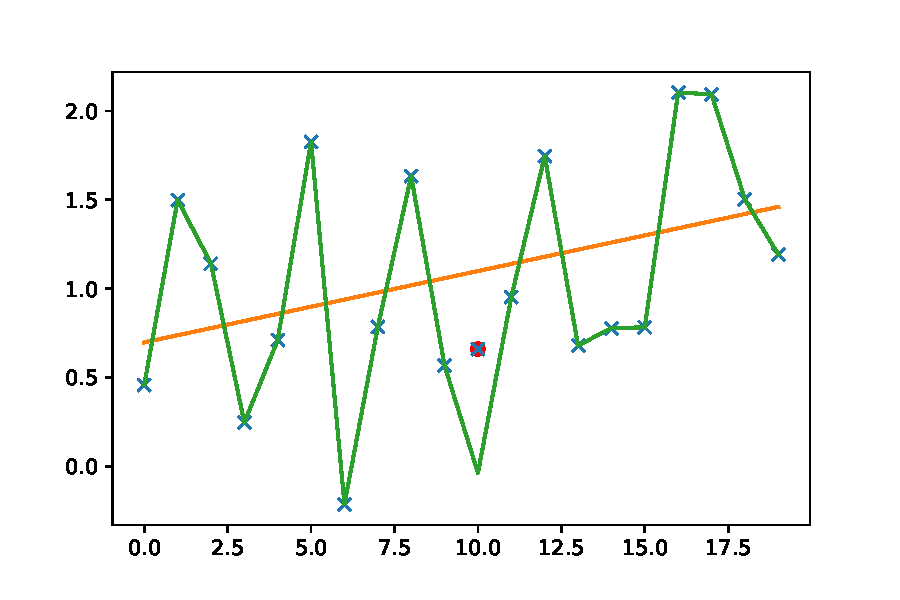
\includegraphics[width=1.0\textwidth]{figures/chapter_4/cross_validation_motivation/fig.pdf}
    \caption{Random data set (blue) with under-fit (orange), and over-fit (green) representations. A particular data point (red) is removed prior to fitting. The removed data point is far from both the over-fit and under-fit representations of the data. }
    \label{cross_validation_motivation}
\end{figure}

Iteration over one suppressed data point is called leave one out cross-validation. It is also possible to leave out any number of data points up to $n-1$, where $n$ is the total number of points in the data set. For leave n out cross validation, one evaluates the solutions generated by every possible way to suppress n data points. This is incredibly computationally expensive. 

In Figure~\ref{cross-validation-example}, the synthetic data set from Figure~\ref{l-curve-example} is reproduced, but $\alpha$ is selected using leave-one-out cross validation. Minimizing the mean-squared error using the cross-validation method suggests $\alpha=7.8\times10^-2.$ This is a different value from what was used in Figure~\ref{cross-validation-example}, but the retrieved spectrum is approximately the same. This suggests a degree of stability across values of $\alpha$ for the application of Tikhonov regularization to the X-ray inversion problem, but testing across many data sets is required for verification. This will be attempted towards the end of this chapter, where the different regularization methods are compared across a large set of synthetic data sets. 

Unlike the ``L-curve'' method, cross-validation leaves no room for the human analysing the problem to have input on the regularization parameter $\alpha$. Instead of looking for an inflection point on a log-log graph, which has some room for interpretation, the minimization of squared errors across values of $\alpha$ for cross-validation is carried out numerically. The minimum located in Figure~\ref{cross-validation-example}, for example, is quite sharply defined. This lack of interpretation is a strength of the cross-validation method. Further, since the minimization process requires no human intervention, it can be  applied to large bodies of synthetic data automatically. This is useful both for running on synthetic data for testing, as well as different sets of experimental data. Since the objective characterization of the performance of an inversion technique to the X-ray inversion problem will depend on its application across to synthetic data, this strength is important. 

\begin{figure}[p]
    \centering
    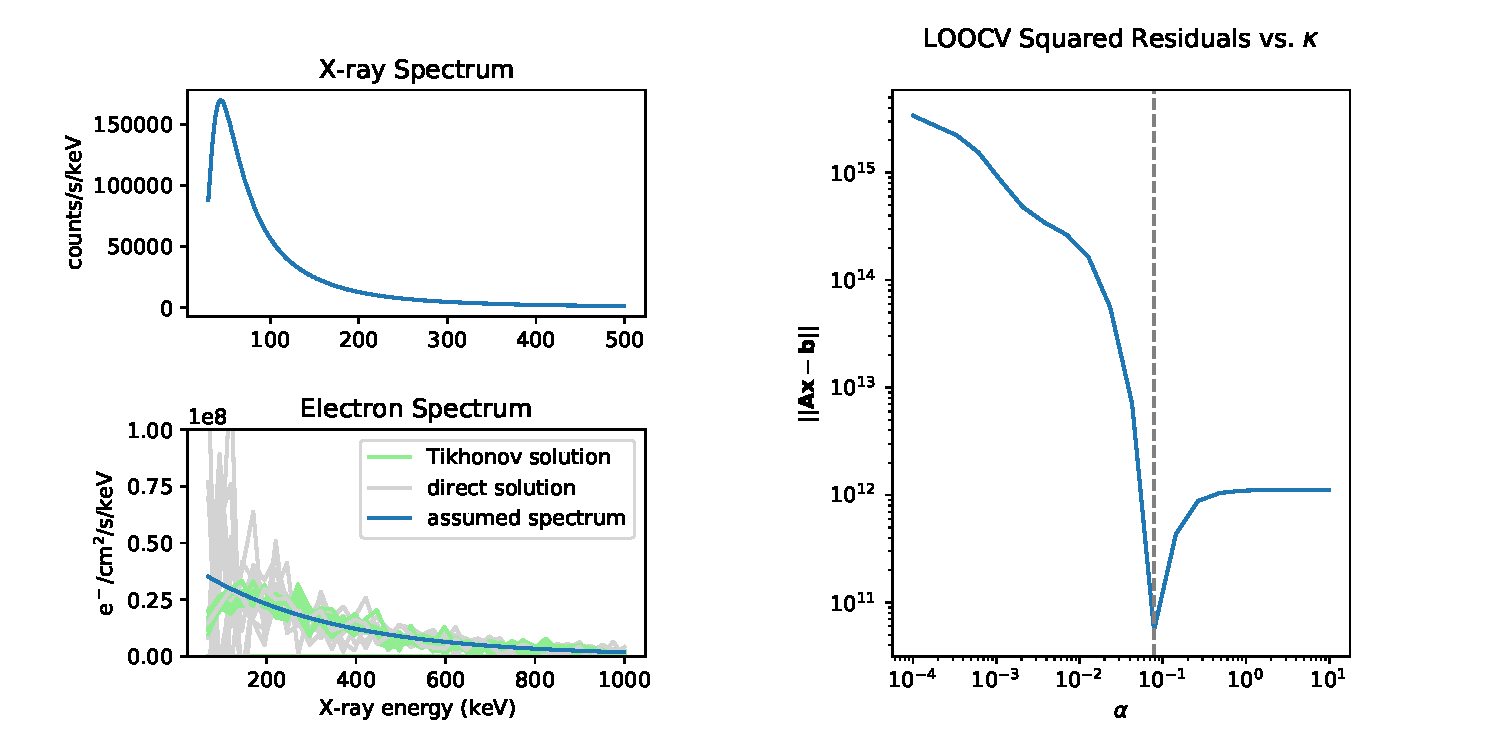
\includegraphics[width=1.1\textwidth]{figures/chapter_4/cross-validation-example/fig.pdf}
    \caption{Application of Tikhonov regularization and the leave-one-out cross-validation method to synthetic exponential electron spectrum. The assumed electron spectrum is shown in blue (bottom, left), and the retrieved spectra are shown for direct inversion (grey) and Tikhonov regularization (green).}
    \label{cross-validation-data}
\end{figure}
\newpage
\section{Higher Order Regularization}

The process of Tikhonov regularization can be interpreted as the addition of a-priori information to the problem. In Tikhonov regularization, the modified least-squares problem:

$$\min_{\mathbf{x}} \vert \vert \mathbf{A} \mathbf{x} - \mathbf{b} \vert \vert + \alpha \vert \vert \mathbf{x} \vert \vert$$

has a penalty term  $\vert \vert \alpha \vert \vert \mathbf{x} \vert \vert$ introduces a preference for solutions with a smaller norm. This was motivated by the fact that more complex solutions typically have a larger number of non-zero terms than simpler solutions, and, to introduce stability, the strength of the regularization should increase with solution complexity. This was indicated graphically through the L-curve method. There are other forms for the penalty term, which can be chosen to align with the properties of physically reasonable solutions to the problem at hand. This section will examine these higher-order regularization terms as applied to the X-ray inversion problem. 

Write a new least-squares problem as:

$$\min_{\mathbf{x}} \vert \vert \mathbf{A} \mathbf{x} - \mathbf{b} \vert \vert + \alpha \vert \vert \mathbf{L} \mathbf{x} \vert \vert$$

where $\mathbf{L}$ is a linear operator. If $\mathbf{L}$ is the identity matrix, then the ordinary regularization is recovered. This is termed zeroth-order tikhonov regularization. In first-order tikhonov regularization, $\mathbf{L}$ is chosen to be the matrix which approximates the first derivative operator:

\[
\mathbf{L} = \begin{bmatrix} 
    1 & -1 & 0 & \dots \\
    0 & 1 & -1 &\dots \\
    \vdots & \ddots & \\
    0 & \dots & 1 & -1 
    \end{bmatrix}
\].

Unlike zeroth-order regularization, which prefers small solutions, this choice of $\mathbf{L}$ penalizes solutions which change - the preference is for constant solutions. For problems where we have an a-priori expectation that solutions are constant, this operator would be the clear choice. A useful and interesting feature of first-order regularization is that no advance knowledge of the best constant solution needs to be applied. 

For the X-ray inversion problem, we do not have any strong expectation that solutions will be constant. In fact, it is more reasonable that electron fluxes decrease as a function of energy. This is motivated by both satellite observations, and balloon flights where models of exponentially decreasing electron spectra tend to best describe measured X-ray data. This motivates the search for a different penalty term for the regularization problem, which better matches this expectation. 

Second-order Tikhonov regularization uses a linear operator which approximates the second derivative:

\[
\mathbf{L} = \begin{bmatrix} 
    1 & -2 & 1 & 0 & \dots \\
    0 & 1 & -2 & 1 & \dots \\
    \vdots & \ddots & \\
    0 & \dots & 1 & -2 & 1 
    \end{bmatrix}
\].

This operator introduces a preference for smooth solutions. There is an intuitive reason why using this operator for the X-ray inversion problem might be useful - as the noise in the measured X-ray spectrum increases, the number of features detectable in the model electron spectrum will go down. A relevant example would be an electron spectrum which is well-described by two beams at different energies. For low noise levels in the corresponding measured X-ray spectrum, the two beams can be resolved through direct inversion, without applying regularization. As the noise in the measured spectrum is increased, second-order regularization will dull and blend the two sharp peaks until eventually they are not distinguishable.  This is a desirable property, since the bias tends towards solutions which reflect the lack of information a high noise measurement represents. This is illustrated in Figure~\ref{two_peak_second_order_example}.

\begin{figure}[p]
    \centering
    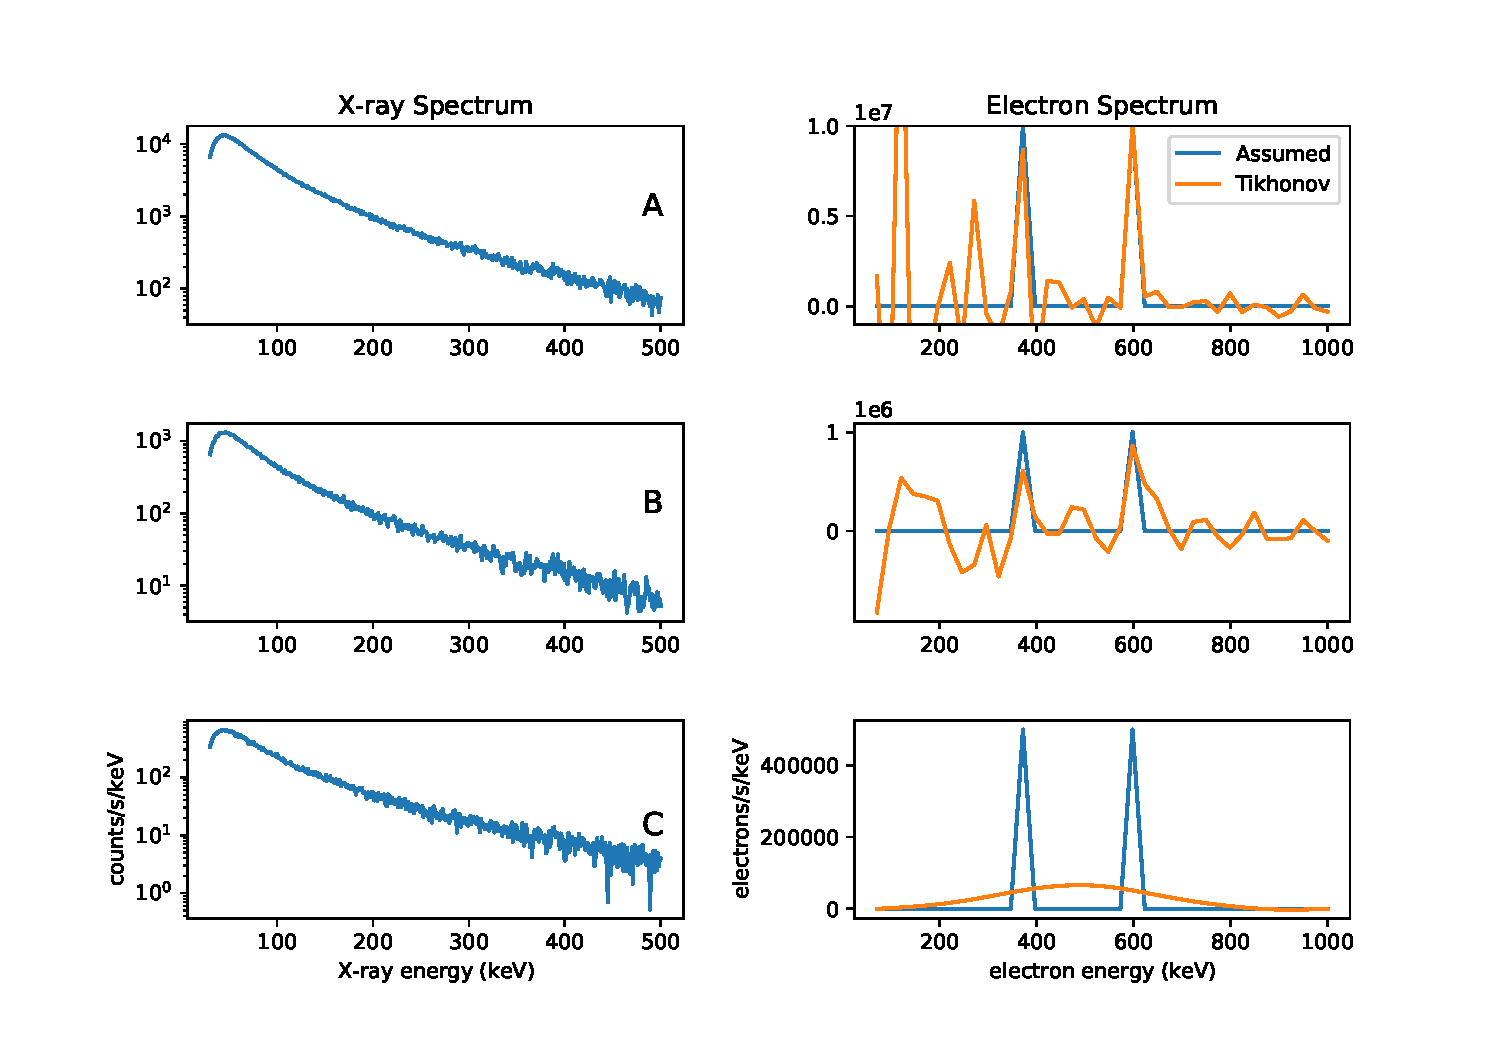
\includegraphics[width=1.1\textwidth]{figures/chapter_4/two_peak_second_order_example/fig.pdf}
    \caption{Application of second-order Tikhonov regularization to synthetic X-ray measurements corresponding to two mono-energetic electron beams at different X-ray fluxes and noise levels (A - $10^7$ electrons / sec / keV, B - $10^6$ electrons / sec / keV, C - $5\times10^5$ electrons / sec / keV)}
    \label{two_peak_second_order_example}
\end{figure}
\newpage

An additional argument for applying second-order Tikhonov regularization to the X-ray inversion problem is that completely sharp, mono-energetic features aren't realistic in natural electron spectra. Thermal processes tend to relax such distributions to have a characteristic width, and over a long enough time period, the central limit theorem tends them towards Gaussian distributions regardless. Since sharp solutions aren't generally expected, it makes sense to choose $\mathbf{L}$ such that they are penalized. This represents further injection of a-priori information to the problem.  

\section{Constraints and Preconditioning}

The application of regularization techniques makes the X-ray inversion problem tractable, with realistic and imperfectly measured input data. In using a biased estimator, we have replaced an impossible linear problem with a condition number approaching $10^{10}$, with a nearby problem that is better behaved. The cost of this is an artificial tendency towards families of solutions influenced by a-priori information, such as smooth solutions, for second-order Tikhonov regularization. The effect of this bias increases with noise in the input data. In this section, we explore methods which can be used to apply simplifying transformations to the X-ray inversion problem prior to the regularization process. Provided that the transformations applied have an inverse, they can be used to re-cast the X-ray inversion problem as an equivalent linear problem in a different space. If the transformations applied are chosen carefully, the equivalent problem can have a condition number which is significantly reduced. This reduces the amount of regularization that needs to be applied for stability, or equivalently, allows more information to be obtained from noisy measurement data. 

As a motivating example, take the linear problem $\mathbf{A}\mathbf{x} = \mathbf{b}$, with $\mathbf{A}$ defined as:

\[
\mathbf{A} = \begin{bmatrix} 
    .0001 & 1.0001 & 0 \\
    0 & 1 & 0 \\
    0 & 0 & 1
    \end{bmatrix}
\].

The condition number of $\mathbf{A}$ is approximately $2.0\times10^{4}$. Instead of calculating $\mathbf{A}^{-1}$, first left and right multiply by linear transformation:

\[
\mathbf{L} = \begin{bmatrix} 
    100 & 0 & 0  \\
    0 & 1  & 0 \\
    0 & 0 & 0
    \end{bmatrix}
\].

The new matrix is:

\[
\mathbf{\tilde{A}} = \begin{bmatrix} 
    1 & 100.01 & 0  \\
    0 & 1  & 0 \\
    0 & 0 & 1
    \end{bmatrix}
\].

with a condition number of $1.0\times10^{4}$. The corresponding transformation can be applied to $\mathbf{b}$ to obtain the solution, $\mathbf{x}$, of the original problem. This preconditioning can be applied before using regularization methods, reducing the amount of regularization required for stability with a  particular problem and data set. 

In general the left and right-multiplication can be done using different matrices. Label the left preconditioner $\mathbf{L}$ and the right preconditioner $\mathbf{R}$. The linear problem:

$$\mathbf{A}\mathbf{x} = \mathbf{b}$$

can then be recast as:

$$(\mathbf{L}\mathbf{A}\mathbf{R}^{-1}\mathbf{R})\mathbf{x} = \mathbf{L}\mathbf{b}.$$

Since the X-ray inversion problem is linear, there is no inherent cost to applying preconditioning methods before solutions are found. Provided matrices $\mathbf{L}$ and $\mathbf{R}$ are not singular, the solution to the original problem can be recovered. 

There is no known general method to determine optimal values for $\mathbf{L}$ and $\mathbf{R}$. There are some specific cases, such as for symmetric matrices, where techniques exist, but the matrix which describes the X-ray inversion problem does not fall into any of these categories. This problem makes finding an appropriate preconditioner for the X-ray inversion problem non-trivial. We will try different combinations of known preconditioners, and stop when a selection is found that significantly reduces the condition number of the problem. 

From a computational perspective, the ``ideal'' matrix representing the X-ray inversion problem would be the identity, with a condition number of one. Compared to the identity matrix, the real matrix representing the X-ray inversion problem has two main undesirable properties. The first is that the rows, which represent X-ray spectra from mono-energetic beams of electrons, have a high degree of col-linearity. This is the main cause of the high condition number of the matrix. The second problem is that the rows and columns have vastly different norms. This is because low energy beams of electrons do not penetrate far into the atmosphere, and their impact in terms of measurable X-rays is small. On the other hand, high energy beams of electrons need only have a small total particle flux to create a very large measurable X-ray response. Figure~\ref{matrix_spectral_plot} (top) shows this for a particular binning scheme on the response matrix though graphs of its rows. The spectrum of singular values is also shown. We will show that preconditioning can have a significant effect on the singular values of the resulting matrix. 

\begin{figure}[p]
    \centering
    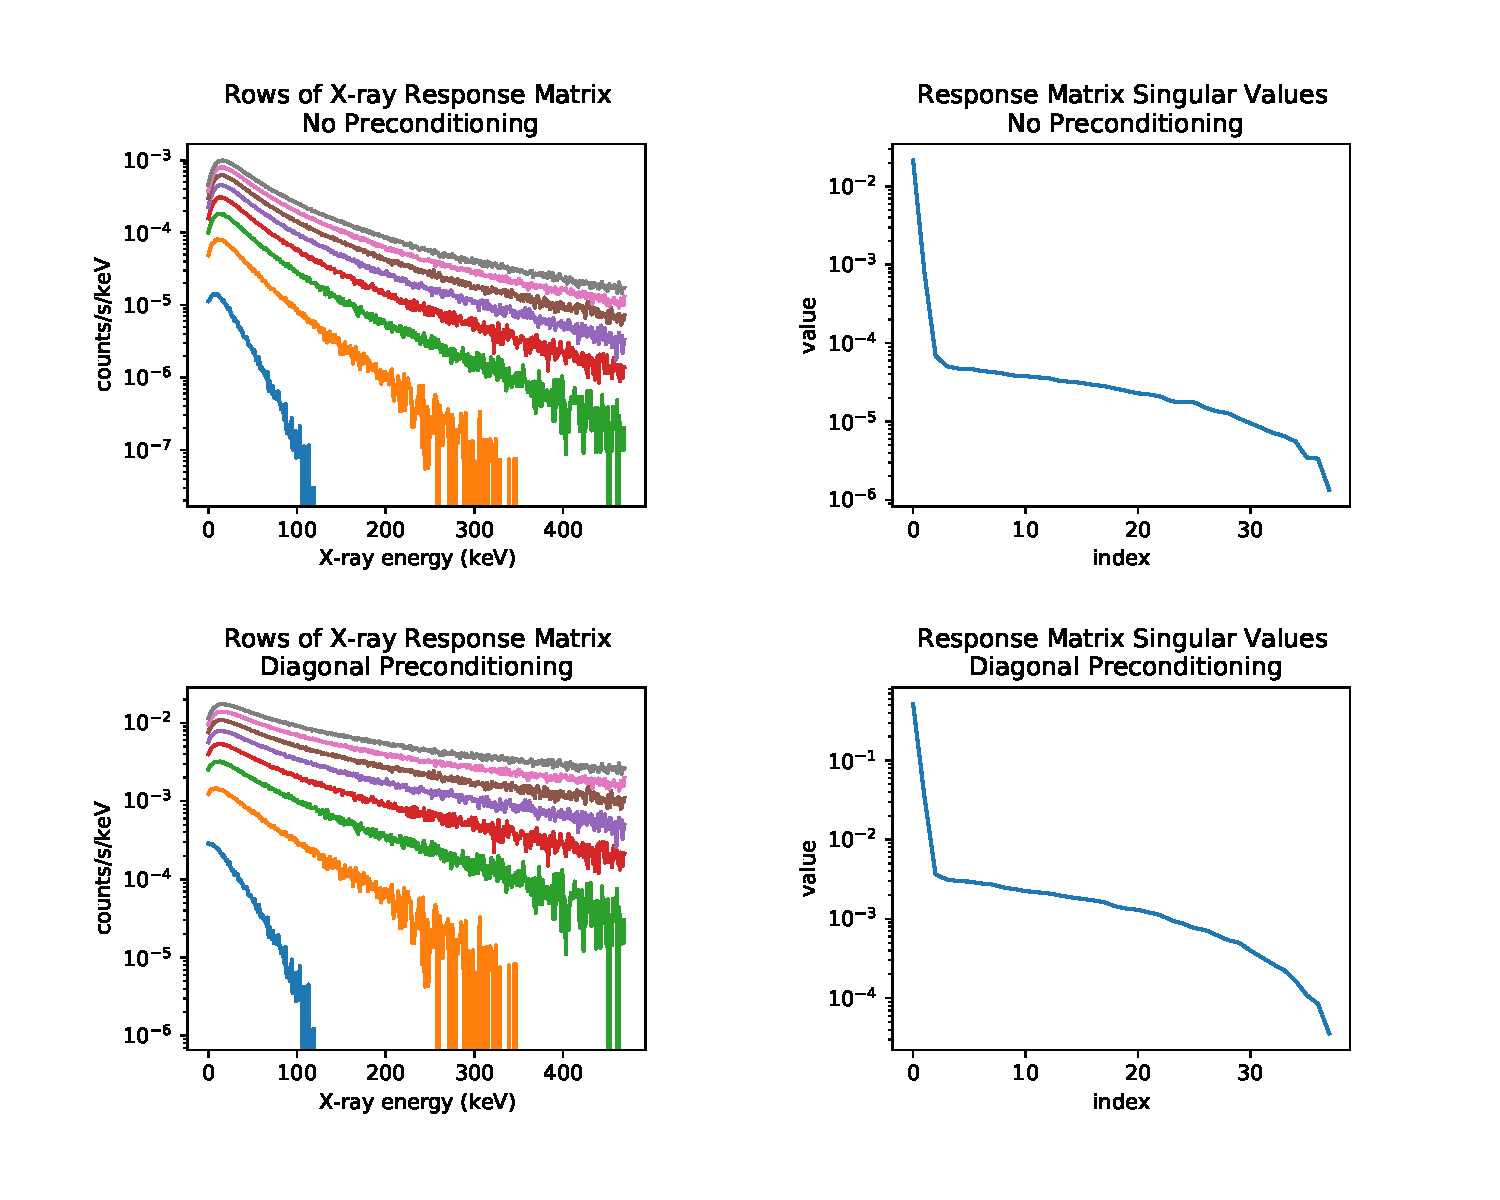
\includegraphics[width=1.1\textwidth]{figures/chapter_4/matrix_spectral_plot/fig.pdf}
    \caption{(left): Graph of the rows of the X-ray response matrix. A high degree of co-linearity is apparent, as with a large scale change between rows. (right): Graph of the singular values of the X-ray response matrix, from largest to smallest. }
    \label{matrix_spectral_plot}
\end{figure}

One classic left-preconditioner is called diagonal scaling. For this preconditioner, a diagonal matrix is constructed such that the entries are equal to the inverse of the norm of the rows of the target matrix. This has the effect of making the row norms of the transformed matrix closer together. Figure~\ref{diagonal_scaling} shows the same 
\appendix
%\fancyhead[RO,LE]{\thepage}
%\fancyfoot{}

\chapter{First Appendix}



\end{document}
